%\chapter{Elements of Scattering Theory - Part II }


\section{Quantum Mechanical Processes} 
\label{scattering-2}

\subsection{The Schr\"odinger Equation}

In quantum mechanics a system is described mathematically by its wave function. The interpretation of the wave function is a complex probability amplitude from which probabilities of outcomes of measurements can be inferred. 

In simpler terms, quantum mechanics postulates that a {\bf free particle} is described by the free Schr\"odinger equation.

The Schr\"odinger equation was formulated in 1925 by Erwin Schr\"odinger and published one year later. For postulating this equation Erwin Schr\"odinger was awarded the Nobel prize in 1933.


The Schr\"odinger's equation is inherently \emph{non-relativistic}. This can be deduced using the operators substitution in the non relativistic energy expression,

    \begin{equation}
        E = \frac{p^2}{2m}.
        \label{eq:classical-energyunpert}
    \end{equation}

Using the relations $E = i\hslash\frac{\partial}{\partial t}$ and $\Vec{p} = -i\hslash\Vec{\nabla}$, which can be summarized in Einstein's notation as

\begin{equation}
\boxed{p_{\mu} = i\hslash \partial_{\mu},}
\end{equation}
then Eq. \eqref{eq:classical-energyunpert} becomes
    \begin{equation}
        -\frac{\hslash^2}{2m}\nabla^2\psi = i\hslash\frac{\partial}{\partial t}\psi.
        \label{eq:schroedinger1unpert}
    \end{equation}

In quantum-mechanical terms, the goal of a scattering experiment is the study of a localized and stationary (time-independent) potential, $V(x)$. Here \emph{localized} implies that $V(x) \rightarrow 0$ when $x \rightarrow \pm \infty$.

For the sake of simplicity, let us just consider the one-dimensional case. The idea is to imagine the scattering experiment as a quantum particle traveling along the $x$-direction and encountering the potential. The equation of motion is governed by the Schr\"odinger equation,

\begin{equation}
\label{eq:schrodinger}
 -\frac{\hslash^2}{2m} \frac{\partial^2 \psi}{\partial x^2} + V(x) \psi =  i\hslash \frac{\partial \psi}{\partial t}.
\end{equation}

The solutions to the Schr\"odinger equation in a single spatial dimension are the {\bf energy eigenstates}
\[\psi(x,t) = e^{\pm \frac{iEt}{\hslash}}\psi(x),\]
where it is clear the separation of the overall wavefunction as the product of a time-dependent and a position-independent term. This holds only if the potential is stationary, i.e. $V=V(x)$.

Negative-energy solutions yield bound states\footnote{This is true only for the Schr\"odinger equation, while the case of a relativistic particle will be different and discussed for the Klein-Gordon equation.}.This can be easily seen with any shape of a one-dimensional potential $V(x)$ where it is assumed that the potential is constant at $x \rightarrow \pm \infty$, meaning that the particle is free far from the region where the potential acts (a typical, reasonable assumption in a scattering experiment). 

Then, by fixing the value of the potential at $x=\pm\infty$ to $0$, it can be seen that initial negative energies will be bound in the region of $x$ where the potential acts ($[x_1,x_2]$), and the particle will oscillate between $x_1$ and $x_2$. Instead, if the initial energy is positive, $E>0$ then a free particle starting from the left with momentum $p$ will be only perturbed by the potential and will then recover its momentum when traveling away from the potential. 

The classification discussed above is interesting, and one could wonder whether in all cases bound states will not appear, even when there is some ``hole'' in the potential. However, even if there is a hole in the potential, the solutions to the Schr\"odinger equation will still be scattering solutions, as the system will be able to tunnel out of the ``hole'' with some non-zero probability.

\subsection{Normalization of the wave function}

In order to be able to interpret the wave function as a description of a physical particle, one needs to consider the problem of its normalisation. From a mathematical point of view, the solutions of the Schr\"odinger equation allow for any normalisation to be chosen; however, this results in different physical interpretations of the meaning of those wave functions.

Let's consider the case of a free particle, which can be described by a plane wave
    \begin{equation}
        \psi = Ne^{i\Vec{p}\cdot\Vec{x}-i\frac{p^2}{2m}t},
    \end{equation}
which solves the Schr\"odinger equation; $N$ is a normalisation factor. Given the probabilistic interpretation of the wave function, a value of \(N\neq1\) implies that a given volume $V$ contains $N^2$ particles,

\begin{equation}
    \int_V | \psi^* \psi| dV = N^2 \times V.
\end{equation}

While the wave function normalisation is a matter of convention, it is important that the physical predictions -- namely, the cross section of a scattering process -- are independent of this choice. Often the choice will be
\begin{equation*}
    \int_V | \psi^* \psi| dV = 1,
\end{equation*}
in which case the wave function will simply be
\begin{equation*}
    \psi = e^{i\Vec{p}\cdot\Vec{x}-i\frac{p^2}{2m}t}.
\end{equation*}

The problem is that, when one considers an infinite volume, it is not possible to fix the wave function normalisation from the normalisation of the total probability (or probability density),%, the probability current is not possible (
as it means that $N^2 \rightarrow 0$. The normalisation of the wave function from the total probability is possible when one considers the free particle not as a single wave function, but rather as a \emph{superposition of plane waves}, i.e. a \emph{wave packet}, which can be written as a Fourier decomposition
   \begin{equation}
        \psi(x) = \int \psi(k) e^{ikx} dk,
    \end{equation}
where
   \begin{equation}
        \psi(k) = \int \psi(x) e^{-ikx} dx.
    \end{equation}

A useful representation of the wave packet is the \emph{Gaussian wavepacket}, which is Gaussian both in momentum and position space and gives a good approximation of the Heisenberg uncertainty relation. For the purpose of these note, we will avoid to enter into the details of this more precise description of a \textbf{quantum particle}.

\subsection{Probability current}

The complex conjugate Schr\"odinger equation can be written as

    \begin{equation}
        -i\frac{\partial}{\partial t}\psi^* + \frac{\hslash}{2m}\nabla^2\psi^* = 0.
        \label{eq:schroedinger2}
    \end{equation}
    
    Multiplying Eq. \eqref{eq:schroedinger1unpert} by $\psi^*$ and Eq. \eqref{eq:schroedinger2} by $\psi$ (on the left side), we obtain
    \begin{equation*}
        i\psi^*\frac{\partial\psi}{\partial t} + \frac{\hslash}{2m}\psi^*\nabla^2\psi = 0, 
    \end{equation*}
    and
    \begin{equation*}
        -i\psi\frac{\partial\psi^*}{\partial t} + \frac{\hslash}{2m}\psi\nabla^2\psi^* = 0.
    \end{equation*}
    Subtracting the two equations we obtain
    \begin{equation*}
        i\left(\psi^*\frac{\partial\psi}{\partial t}+\psi\frac{\partial\psi^*}{\partial t}\right) + \frac{\hslash}{2m}\left(\psi^*\nabla^2\psi - \psi\nabla^2\psi^*\right) = 0,
    \end{equation*}
    which becomes
    \begin{equation}
        i\frac{\partial}{\partial t}(\psi^*\psi) + \frac{\hslash}{2m}\Vec{\nabla}\cdot(\psi^*\Vec{\nabla}\psi - \psi\Vec{\nabla}\psi^*) = 0.
        \label{eq:density-prob-continuity}
    \end{equation}
    The quantity $\rho = \psi^*\psi$ is the probability density. Equation \ref{eq:density-prob-continuity} is the usual continuity equation.
    
    If we consider a volume $V$, the variation of probability in the volume can be expressed as 
    \begin{equation*}
        \delta p = \frac{\partial}{\partial t}\iiint_{V} \rho\,dV.
    \end{equation*}
    If we call $\Vec{j}$ the vector of the probability current, we can write the probability flux through a surface element $\Vec{ds}$ as $\Vec{j}\cdot\Vec{dS}$ (as shown in Figure \ref{fig:probability-current}. We exploit the divergence theorem to write
    \begin{equation*}
        \frac{\partial}{\partial t}\iiint_{V} \rho \,dV = -\oiint_{S} \Vec{j}\cdot\Vec{dS} = \iiint_V \Vec{\nabla}\cdot\Vec{j} \,dV.
    \end{equation*}
    \begin{figure}
        \centering
        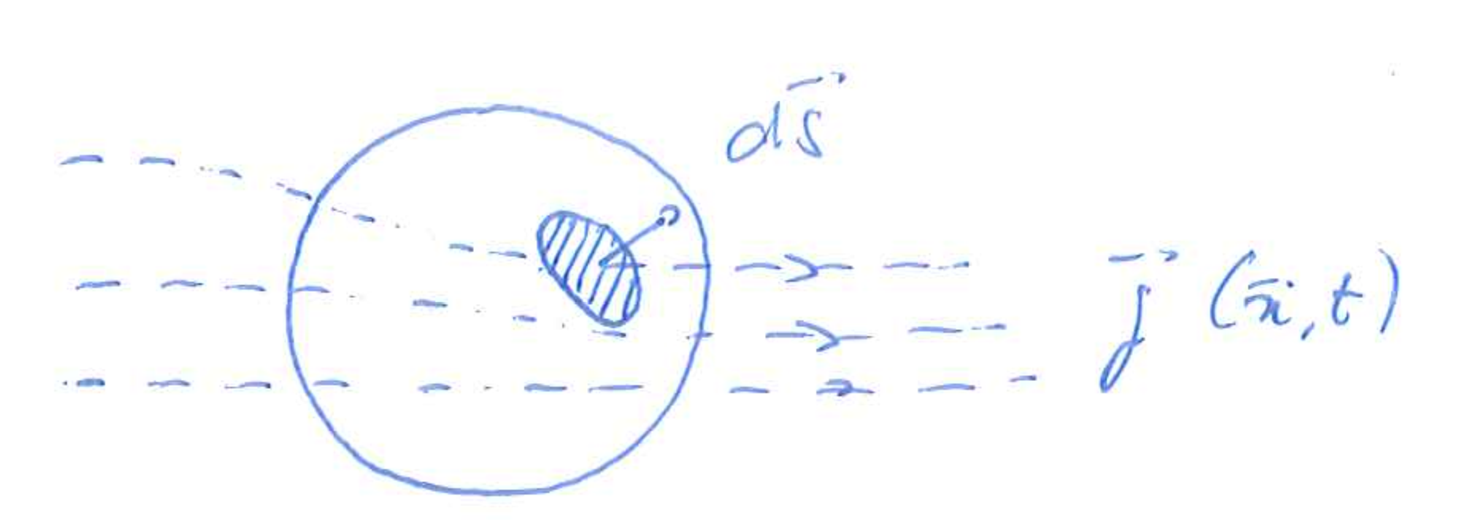
\includegraphics[width=0.7\textwidth]{Figures/probability-current}
        \caption{Representation of the probability flux.}
        \label{fig:probability-current}
    \end{figure}
    This equations holds for each arbitrary choice of $V$, therefore we can write
    \begin{equation*}
        \frac{\partial}{\partial t}\rho + \Vec{\nabla}\cdot\Vec{j} = 0,
    \end{equation*}
    and identify this probability current with the expression of Eq. \eqref{eq:density-prob-continuity}, obtaining
    \begin{equation*}
        \Vec{j} = \frac{\hslash}{2mi}\left(\psi^*\Vec{\nabla}\psi - \psi\Vec{\nabla}\psi^*\right).
    \end{equation*}
    
    If we take the free-particle wave function and choose to normalise it by $N$, where $N^2$ has the meaning of number of particles in a volume $V$, then we  have $\rho = \psi^*\psi = N^2$, and the current $\Vec{j}$ will be  given by
    \begin{equation*}
        \Vec{j} = \frac{1}{2mi}\left(\psi^*(i\Vec{p}\psi)-\psi(i\Vec{p})\psi^*\right) = \frac{\Vec{p}}{2m}2\left|\psi\right|^2 = \frac{\Vec{p}}{m}\left|\psi\right|^2 = \Vec{v}\cdot \rho,
    \end{equation*}
    where we used \(\Vec{p}=-i\hslash\Vec{\nabla}\) and \(\nabla\psi^*=(\nabla\psi)^*=(\frac{\Vec{p}}{i\hslash}\psi)^*=\frac{\Vec{p}}{-i\hslash}\psi^*\).
    We can conclude that, since $\rho = |N|^2$ is the density (number of particles per unit volume),  then $\Vec{j} = \rho\Vec{v}$ is the flux of particles through an unit arc in a unit time. We will see that this is the same expression as defined in the cross section formula calculation with the Fermi's golden rule.


\subsection{Time independent formalism, the one dimensional case}

Let us consider the case of a generic (stationary) potential $V(x)$, such as the one illustrated in Figure~\ref{fig:potential-1}, and a system consisting of a particle in one dimension. The  Schr\"odinger equation is a second order differential equation and has two generic solutions, which correspond to the particle moving from right to left or from left to right. The possible states at infinity, which would correspond to the initial and final states being free particles, will have energy

\[ E = \frac{\hslash^2 k^2}{2m}.\]

The scattering states (i.e. those with $E>0$) give rise to solutions that can be right-moving, $e^{ikx}$, or left-moving, $e^{-ikx}$.\footnote{We must stress that, since the Hamiltonian is time-independent by hypothesis, here we are not talking about time dependence at all: the state of the system does not evolve in time.}

    \begin{figure}
%        \centering
        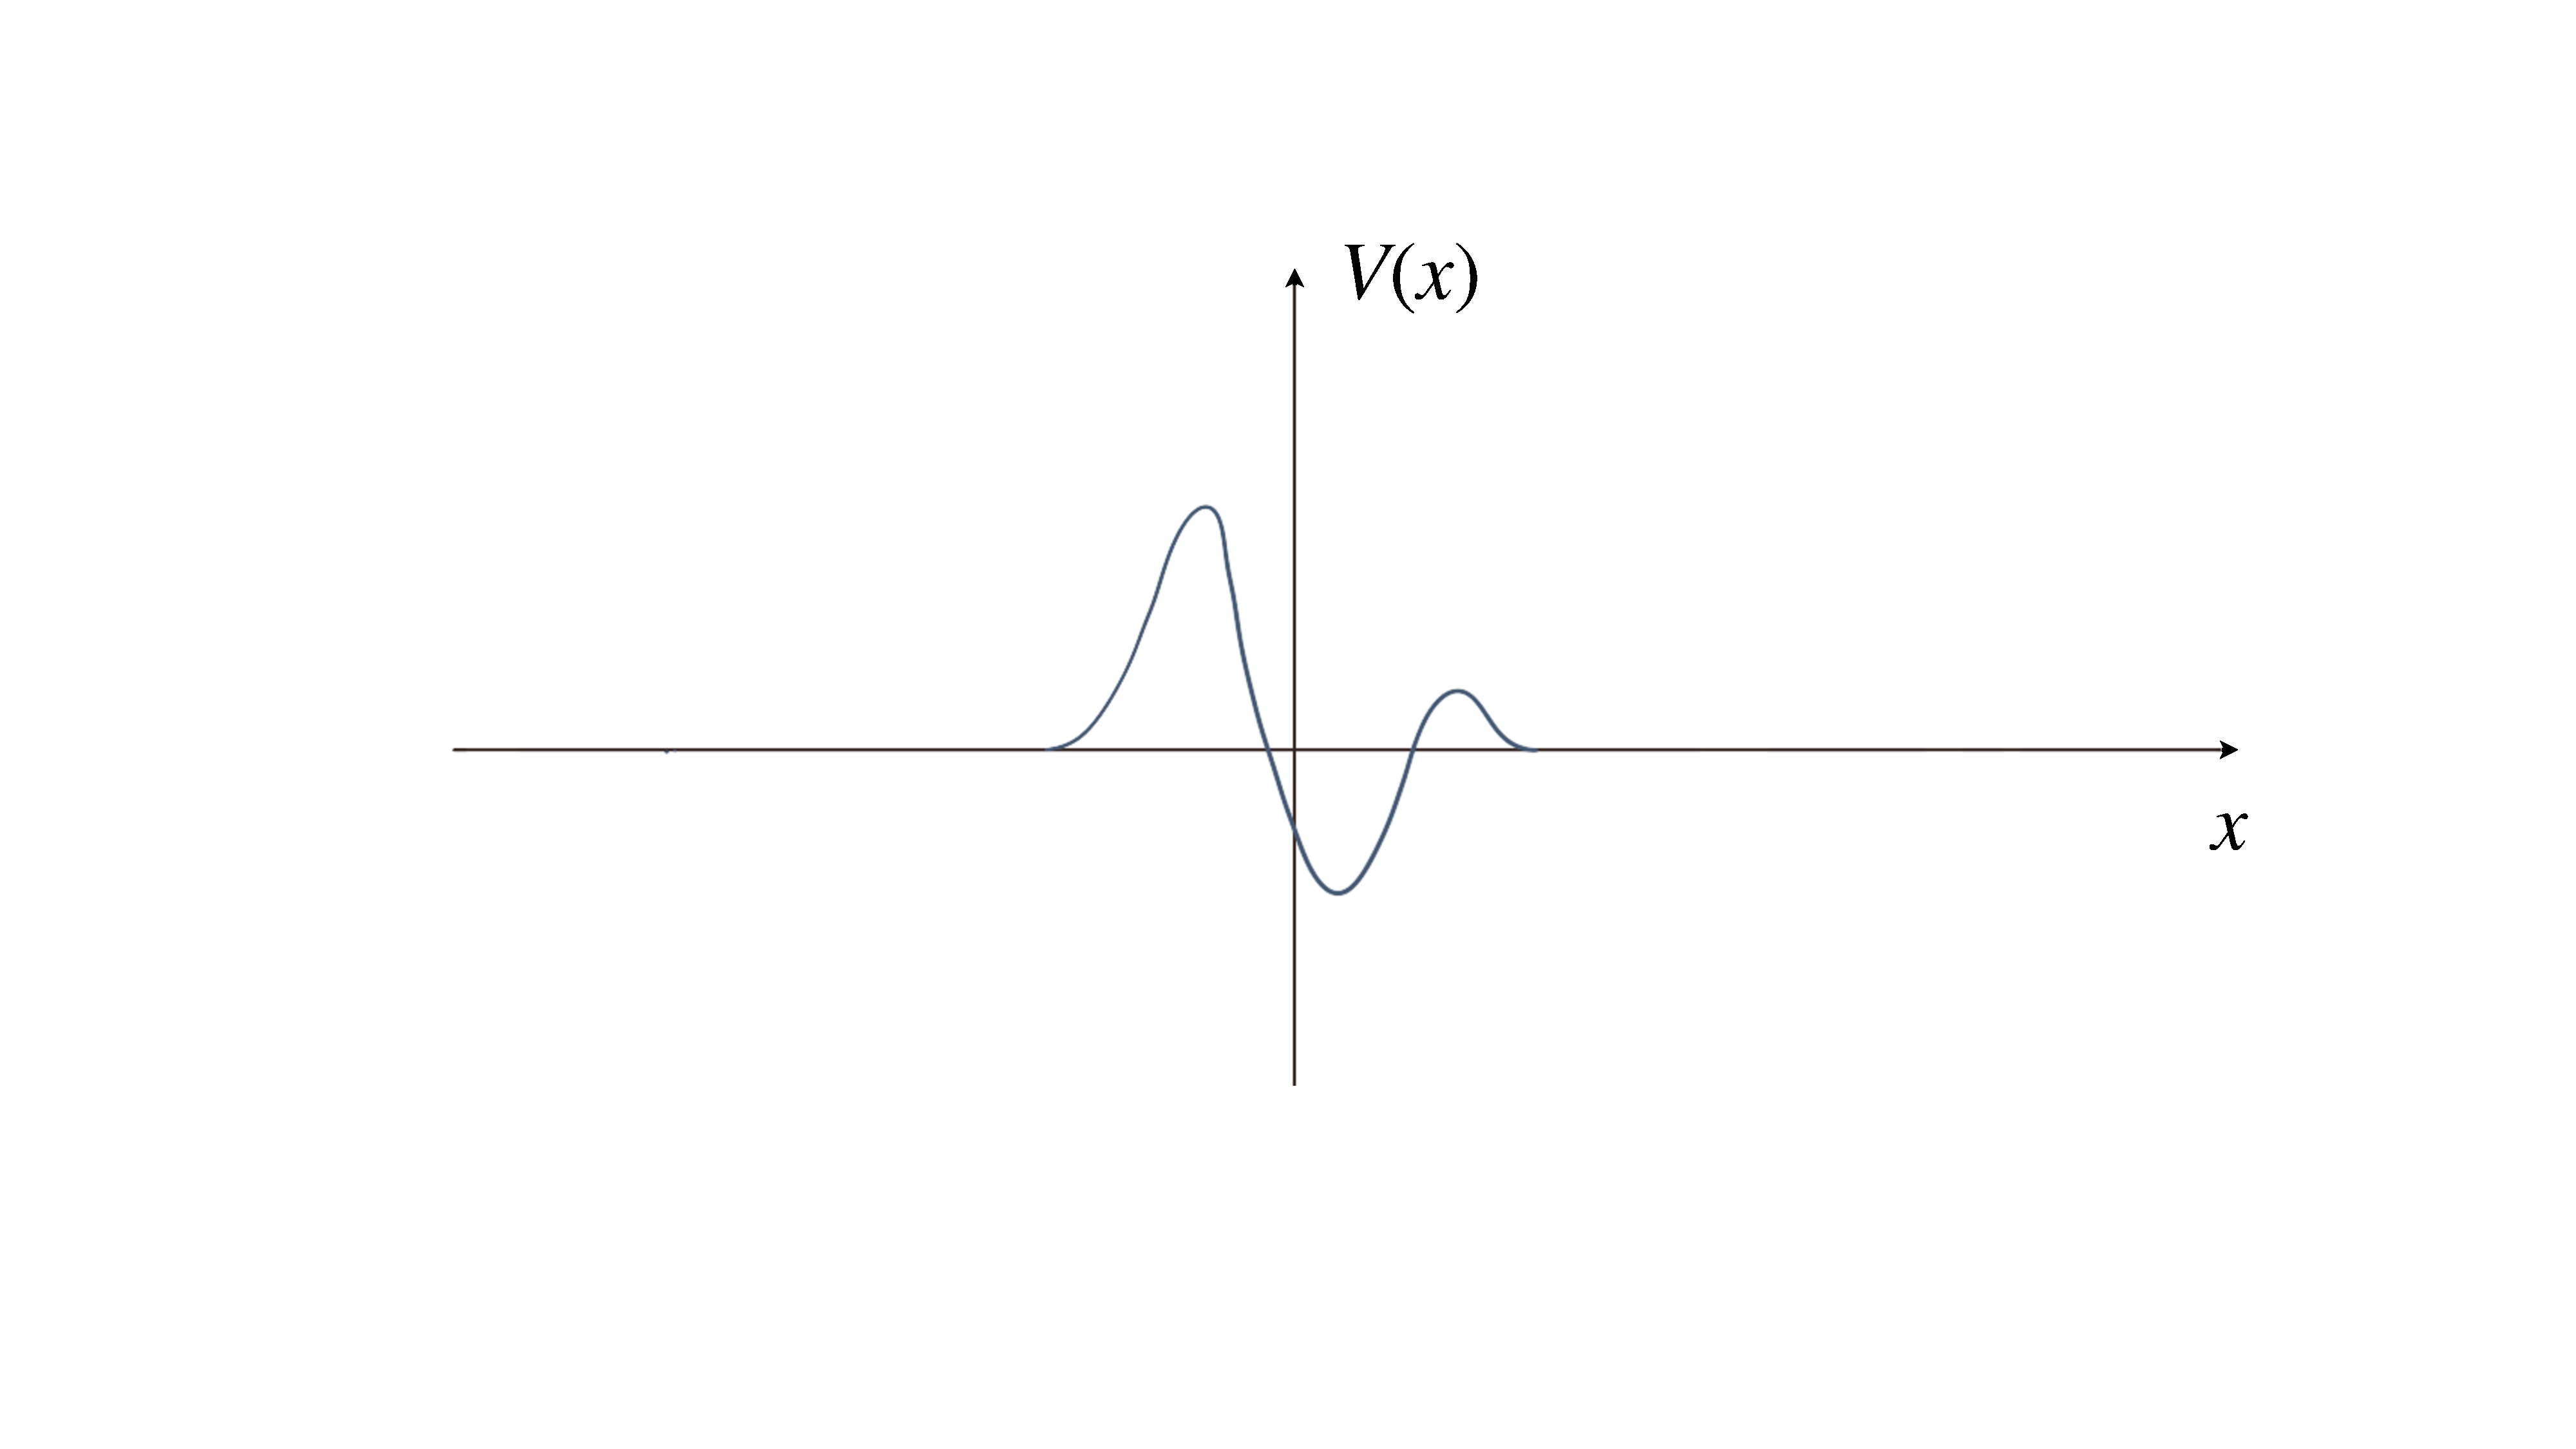
\includegraphics[width=0.7\textwidth]{Figures/Potential-1}
        \caption{Illustration of a one-dimensional potential which is vanishing at large values of $x$ far from the localized region where the potential is non-zero.}
        \label{fig:potential-1}
    \end{figure}


One can calculate the various probabilities of scattering by seeking solutions that are free particles at $x \rightarrow \pm \infty$: the resulting wave functions will be a combination of the two types of solutions (right-moving and left-moving). The problem is then posed in a stationary fashion, and we will look for solutions $\psi(x)$ of the form of a particle probing the potential from left to the right,
\begin{equation}
\psi_L(x) = \left \{ 
    \begin{matrix}
 e^{ikx} + r e^{-ikx}  \\
 t e^{ikx} 
\end{matrix}
    \right . \; \; \; \; 
    \begin{matrix}
 x \rightarrow -\infty  \\
 x \rightarrow +\infty 
\end{matrix}
\end{equation}
where $r$ and $t$ are complex numbers which will be referred to as {\it reflection} and {\it transmission} amplitudes. 

While the scattering process is inherently a time-dependent concept, here we are modeling the scattering by a system of plane waves. It could be thought of as a beam of particles thrown towards the potential from the left, with part of the beam being reflected and part being transmitted.

Taking the simple example of a plane wave for the free particle, for its interpretation in terms of number of particles and probabilities it is useful to compute the probability current,

\[ j = \frac{i\hslash}{2m} (\psi^* \frac{\partial \psi}{\partial x} -  \frac{\partial \psi^*}{\partial x} \psi.)\]

By simply replacing the wave function solutions in this equation yields on the left ($x \rightarrow -\infty$)
\begin{eqnarray*}
j & = & \frac{\hslash}{2im} [(e^{-ikx}+r^* e^{ikx})(ike^{ikx}-ikr e^{-ikx})-(e^{ikx}+r e^{-ikx})(-ike^{-ikx}+ikr^* e^{ikx})] \\
& = & \frac{\hslash k}{2m} [ 1 -r e^{-i2kx} + r^* e^{i2kx} -rr^* +1 - r^*e^{i2kx} + re^{-i2kx} - r r^*] \\
& = & \frac{\hslash k}{m} (1 - |r|^2 ).
\end{eqnarray*}
On the right instead ($x \rightarrow +\infty$) one gets
\[ j = \frac{\hslash}{2im} ik ( t^*t + t t^* ) = \frac{\hslash k}{m} |t|^2.\]
The conservation of the probability current yields
\[|r|^2 + |t|^2 = 1,\]
where $R = |r|^2$ and $T = |t|^2$ can be interpreted as the probabilities of reflection and transmission respectively, where on the left there is the sum of two fluxes of particles, one which is propagating towards the right with a flux of $T$ and velocity $+k/m$ and a flux of particles moving to the left with a flux $R$ with a velocity $-k/m$, while on the right side the transmitted particles for a beam of flux $T$ with a velocity $+k/m$. 

This is the so-called case of ``scattering from the left''. The same can be done for the case of the scattering from the right, where the problem is posed in the following terms (a beam of particles coming from the right):
\begin{equation}
\psi_R(x) = \left \{ 
    \begin{matrix}
 e^{-ikx} + r' e^{ikx}  \\
 t' e^{-ikx} 
\end{matrix}
    \right . \; \; \; \; 
    \begin{matrix}
 x \rightarrow +\infty  \\
 x \rightarrow -\infty 
\end{matrix}
\end{equation}

From this we can note that there is a simple ``mirror'' relation between the case of the scattering from the left and the scattering from the right. Since the potential $V(x)$ is real, then $\psi_L^*$ is also a solution of the Schr\"odinger equation, 
\[ -\dfrac{\hslash^2}{2m} \dfrac{\partial^2 \psi}{\partial x^2} = (E-V(x)) \psi, \]
in the form
\begin{equation}
\psi_L^*(x) = \left \{ 
    \begin{matrix}
 e^{-ikx} + r^* e^{ikx}  \\
 t^* e^{-ikx} 
\end{matrix}
    \right . \; \; \; \; 
    \begin{matrix}
 x \rightarrow -\infty  \\
 x \rightarrow +\infty 
\end{matrix}
\end{equation}

We then recognize that
\begin{equation}
\dfrac{\psi_L^*(x) -r^* \psi_L(x)}{t^*}  = \left \{ 
    \begin{matrix}
 (1-|r|^2) e^{-ikx} /t^* = |t|^2 e^{-ikx} / t^* = t e^{-ikx} \\
 t^* e^{-ikx} -r^* t e^{ikx} = e^{-ikx} -r^* \dfrac{t}{t^*} e^{ikx} 
\end{matrix}
    \right . \; \; \; \; 
    \begin{matrix}
 x \rightarrow -\infty  \\
 x \rightarrow +\infty 
\end{matrix}
\end{equation}

which is in the same form as the solution for the scattering from the right, if we take $t = t'$ and $r'= r \frac{t}{t^*}$. This is a very interesting result that shows that the transition amplitude is the same {\bf irrespective of the shape of the potential} and that the reflection only differs by a phase. The transmission and reflection probabilities $R$ and $T$ are thus the same in the scattering from the left and in the scattering from the right.

\subsection{Scattering in three dimensions and scattering amplitudes}
In the much more realistic case of a three dimensional potential localised in space, a similar stationary formalism can be applied. In this case the incoming beam of particles is represented by a plane wave, or a beam of particles with a given momentum and in the $z$ direction ($\psi(\vec{r}) = e^{ikz}$). The scattered particles will then be represented by a spherical wave with a given scattering amplitude which depends on the scattering direction $\psi(\vec{r}) =  f(\theta,\phi) \frac{e^{i\vec{k}.\vec{r}}}{r}$. The dependence in $1/r$ of the scattered wave function is obtained as a result of solving the Schr\"odinger equation and can be simply interpreted in terms of density of states as $|\psi|^2$ will be expanding over a sphere of surface proportional to $r^2$. The resulting overall wave function will then be  written as
\begin{equation}
\label{eq:scat-3d}
    \psi(\vec{r}) = e^{ikz} + f(\theta,\phi) \frac{e^{i\vec{k}.\vec{r}}}{r}.
\end{equation}
In this case the probability current can be expressed as
\[ \vec{j} = \frac{\hslash}{2im} (\psi^* \nabla \psi -  \psi \nabla \psi^*  ) \]
The current can also be separated into an incident current obtained from the incident ($e^{ikz}$) part of the wave function,
\[\vec{j}_{incident} =  \frac{\hslash k}{m} \hat{z},\]
which can be seen as a beam of particles with velocity $\hslash k/m$ along the $z$ direction. We will derive the scattered current in a given direction in space $(\theta,\phi)$ under the assumption that the potential is central (i.e. that it does not depend on $\phi$), and neglecting the $1/r^2$ terms from the derivative in terms of the polar angle $\theta$, which are suppressed as $1/(r \sin \theta) \partial f \partial \theta$ and the derivative of $1/r$. One gets\footnote{We started from \[ \nabla = \pd{}{r} \hat{r} + \frac{1}{r}\pd{}{\theta}\hat{\theta}+\frac{1}{r\sin\theta}\pd{}{\phi}\hat{\phi}.\]The derivative in $\phi$ in the last term will have no effect as the potential is central, and so we immediately see that \[\nabla\psi = \nabla\left(\frac{1}{r}f(\theta,\phi)e^{i\vec{k}\cdot\vec{r}}\right)= \pd{\psi}{r}\hat{r}+\mathcal{O}\left(\frac{1}{r^2}\right)\].}
\[\vec{j}_{scattered} \sim  \frac{\hslash k}{m} \frac{|f(\theta)|^2}{r^2}\hat{r} + \mathcal{O}\left(\frac{1}{r^3}\right)\]

If we then consider the flux of particles across an element area $dA$ in space, which spans a solid angle $d\Omega = dA/r^2$, then we have
\[\vec{j}_{scattered} \cdot \hat{r} \, dA =  \frac{\hslash k}{m} |f(\theta)|^2 d\Omega.\]
Taking the ratio of the scattered flux to the incident beam flux will thus give the differential cross section $d\sigma$,
\[ d\sigma = \frac{\vec{j}_{scattered}}{\vec{j}_{incident}} = \frac{\hslash k |f(\theta)|^2 /m d\Omega}{\hslash k /m}
 = |f(\theta)|^2 d\Omega, \]
while the differential cross section can then be expressed as
\[ \frac{d\sigma}{d\Omega} = |f(\theta)|^2 .\]We have therefore seen that the scattering amplitude and the differential cross section are linked together.
 
\subsection{Partial waves} \label{sec:partialwaves}
In a central potential, i.e. which does not depend on $\phi$, it is interesting to seek solutions of the Schr\"odinger equation (similarly to the resolution of the Hydrogen atom) in terms of spherical harmonics. We start from the fact that the Laplacian operator $\nabla^2$ can be written, in spherical coordinates\footnote{We have
\[ \vec{r}=\begin{cases}x = r \sin\theta \cos\phi\\ y = r \sin\theta \sin\phi\\ z = r \cos\theta\end{cases}\]
and the unit vectors are 
\[ \begin{cases}\hat{r}=\frac{d\vec{r}/dr}{|d\vec{r}/dr|} = \frac{(\sin\theta\cos\phi, \sin\theta\sin\phi,\cos\theta)}{\sqrt{(\sin\theta\cos\phi)^2+(\sin\theta\sin\phi)^2+(\cos\theta)^2}}=(\sin\theta\cos\phi,\sin\theta\sin\phi,\cos\theta)\\
\hat{\theta}=\frac{d\vec{r}/d\theta}{|d\vec{r}/d\theta|} = \frac{(r\cos\theta\cos\phi, r\cos\theta\sin\phi,-r\sin\theta)}{r}=(\cos\theta\cos\phi,\cos\theta\sin\phi,-\sin\theta)\\
\hat{\phi}=(-\sin\phi,\cos\phi,0)\\
\end{cases}\]
thus
\begin{align*}
    \pd{\hat{\theta}}{\phi} &= (-\cos\theta\sin\phi, \cos\theta\cos\phi, 0) = \cos\theta\hat{\phi},\\
    \pd{\hat{\phi}}{\theta}&=0,\\
    \pd{\hat{\phi}}{\phi}&=(-\cos\phi, -\sin\phi, 0).
\end{align*}
}, as
\begin{eqnarray*}
 \nabla^2 &=  \dfrac{1}{r^2} \dfrac{\partial}{\partial r} \left( r^2 \dfrac{\partial}{\partial r} \right) + \dfrac{1}{r^2 \sin \theta} \dfrac{\partial}{\partial \theta}  \left( \sin \theta \dfrac{\partial}{\partial \theta} \right) + \dfrac{1}{r^2 \sin^2 \theta}   \left( \dfrac{\partial^2}{\partial \phi}  \right) \\ 
    & =  \dfrac{1}{r^2} \dfrac{\partial}{\partial r} \left(r^2 \dfrac{\partial}{\partial r} \right) - \dfrac{\vec{L}^2}{\hslash^2 r^2},
\end{eqnarray*}
where we used the fact that the partial derivative in $\phi$ will have no effect, and that $\vec{L}^2 = (\vec{r} \times \vec{p})^2 = (\vec{r} \times  -i\hslash \nabla)^2$. With a bit of math (in which we simply took into account how the derivatives of the unit vectors are written, cf. footnotes), we get
\begin{equation}\label{eq:ellequadro}\vec{L}^2 = -\hslash^2\left [ \dfrac{\partial^2}{\partial \theta^2} + \dfrac{1}{\tan \theta} \dfrac{\partial}{\partial \theta} + \dfrac{1}{\sin^2 \theta}\dfrac{\partial^2}{\partial \phi^2}  \right ].\end{equation}
 
The  Schr\"odinger equation $E\psi=-\hslash^2/2m\nabla^2\psi+V\psi$ in a central potential  $V(r)$ can then be written as
\[ E \psi = -\frac{\hslash^2}{2m} \frac{1}{r^2} \frac{\partial}{\partial r} \left ( r^2 \frac{\partial}{\partial r} \right ) \psi  +  \frac{\vec{L}^2}{2 m r^2} \psi +V(r) \psi.\]
Similarly to the case of the hydrogen atom, we can solve this equation via separation of variables, by expressing the wave function as the product between a radial wave function $R(r)$ and an angular wave function $P_l(\theta)$ (given the assumption of a central potential and therefore no $\phi$ dependence). We obtain
\begin{eqnarray}
\label{eq:SchrodingerSpherical}
E\psi(r,\theta)=E R(r) P_l (\theta) = & -\dfrac{\hslash^2}{2m} P_l(\theta) \frac{1}{r^2} \dfrac{\partial}{\partial r} \left ( r^2 \dfrac{\partial}{\partial r} \right ) R(r) \nonumber \\  & +  R(r)\dfrac{\vec{L}^2}{2 m r^2} P_l(\theta) + V(r) R(r) P_l (\theta),
\end{eqnarray}
where the index $l$ was conveniently introduced as we already know that the angular part of the wave function will be solved with Legendre polynomials. Having restricted ourselves to $\phi$-independent solutions, the Schr\"odinger equation separates into two equations, an angular and a radial one. The angular part is
\[\vec{L}^2 P_l(\theta) = \hslash^2 l(l+1) P_l(\theta)\]
which can then be written in terms of $w = \cos \theta$ and therefore $ d w   = - \sin \theta d\theta$, from which one can write \(\partial f/\partial \theta=\partial f/\partial w\cdot \partial w/\partial \theta\) and get
\[ \dfrac{\partial f}{\partial \theta^2} = \dfrac{\partial }{\partial \theta} \left (  -\sin \theta \dfrac{\partial f}{\partial w} \right ) = - \cos \theta \dfrac{\partial f}{\partial w} + \sin^2 \theta \dfrac{\partial^2 f}{\partial w^2} = - w \dfrac{\partial f}{\partial w} + (1-w^2) \dfrac{\partial^2 f}{\partial w^2}.\]
One can then replace these expressions for the first and second order derivatives in $\theta$ in Eq. \eqref{eq:ellequadro} to write the angular equation as
\[  \boxed{ \dfrac{\partial}{\partial w} (1-w^2) \dfrac{\partial}{\partial w} P_l(w)  + l(l+1) P_l(w) =0 },\]
where we wrote with no loss of generality the eigenvalue of the \(\vec{L}^2\) operator as \(l(l+1)\).

In the separation of variables, using the constant $\hslash^2 l(l+1)$, from Eq.~\eqref{eq:SchrodingerSpherical} the radial equation will become:
\begin{eqnarray*}
[E -V(r)]  R(r) P_l(\cos \theta) & = & -\dfrac{\hslash^2}{2m} P_l(\cos \theta) \dfrac{1}{r^2} \dfrac{\partial}{\partial r} \left ( r^2 \dfrac{\partial}{\partial r} \right ) R(r) \\
& & + \dfrac{\hslash^2 l(l+1)}{2mr^2} R(r) P_l (\cos \theta), %+ V(r) R(r) P_l (\cos \theta)
\end{eqnarray*}
which reduces to
\[ [E -V(r)]  R(r) = -\frac{\hslash^2}{2mr^2}  \frac{1}{r^2} \frac{\partial}{\partial r} \left ( r^2 \frac{\partial}{\partial r} \right ) R(r) + \frac{\hslash^2 l(l+1)}{2mr^2} R(r).\]

If we take the expression of the (non-relativistic) kinetic energy, and define the normalised potential $\tilde{V}(r)$ as
\[ E = \dfrac{\hslash^2 k^2}{2m}  \; \; \; \; {\rm and} \; \; \; \; \tilde{V}(r) = \dfrac{2m}{\hslash^2} V(r), \]
then the radial part of the Schr\"odinger equation can be written as
\[\boxed{ \left [  \dfrac{\partial^2}{\partial r^2} + \dfrac{2}{r}  \dfrac{\partial}{\partial r} - \dfrac{l(l+1)}{r^2} - \tilde{V}(r) + k^2 \right ] R_l(r) = 0}.\]

As we had anticipated with the introduction of the index $l$, we can recognise  $P_l$ as the Legendre polynomials, which are eigenstates of the angular momentum operator $\vec{L}^2$ and thus solutions of the angular part of the Schr\"odinger equation.

The {\bf partial wave} expansion consists in writing a generic wave function as a linear combination of partial waves, each of which is a solution of the Schr\"odinger equation in the separation of variables:
\begin{equation}
    \psi = \sum_{l=0}^{\infty} R_l(r) P_l (\cos \theta)).
\end{equation}

In absence of a potential, the free particle system will correspond to $\tilde{V}(r) = 0$ and therefore the radial equation can be written as

\[\left [ \dfrac{\partial^2}{\partial r^2} - \dfrac{l(l+1)}{r^2} + k^2 \right ] (r R_l(r)) = 0.\]

The solutions to this equation are the {\it Bessel spherical functions} %(see Appendix~\ref{appendix:bessel}),
. It can be seen that for $l=0$ the solution is very simple,
\[R_0(r) = \dfrac{e^{\pm i kr}}{r},\]
i.e. ingoing (outgoing) a plane wave, depending on the sign $\pm$.

Again, when far away from the region where the potential is non-vanishing, we must  also seek for the plane wave solutions as the {\it incident} wave function
\[ \psi_{incident}(\vec{r}) = e^{i kr \cos \theta}  \]
Now, let's express the plane wave in terms of partial wave expansion, i.e. in the form
\begin{equation}\label{eq:eikappazeta}
  e^{ikz} = e^{ikr \cos \theta} = \sum_{l=0}^{\infty} R^p_l(r) P_l (\cos \theta).
\end{equation}
We can use the properties of Legendre polynomials, such as their orthogonality, which can be expressed in the integral form
\[\int_{-1}^{1} P_l(x)P_m(x) dx = \dfrac{2}{2l+1} \delta_{ml},\]
From this we can easily write $R^p_l(r)$ in a simple form. Let's multiply both terms of Eq. \eqref{eq:eikappazeta} by $P_m(\cos\theta)$, and integrate in $dw=d(cos\theta)$: we get
\[
\int_{-1}^1 dw P_m(w) e^{ikrw} =\int_{-1}^1\sum_{l=0}^\infty dw R_l^p(r)P_l(w) = \frac{2}{2m+1} R_m^p(r).
\]
Thus we have (we change label from $m$ to $l$)
\begin{eqnarray}
R^p_l(r) & = & \dfrac{2l+1}{2} \int_{-1}^1 dw P_l(w)e^{ikrw} \nonumber \\
%\sum_{m=0}^{\infty} R^p_m(r) \int_{-1}^{1}  P_m (w)P_l (w) dw) \nonumber \\
%& = & \dfrac{2l+1}{2} \sum_{m=0}^{\infty} R^p_m(r) \delta_{lm}) \nonumber \\
%& = &  \dfrac{2l+1}{2} \int_{-1}^{1} e^{ikr w} P_l(w) dw \nonumber  \\
& = & \dfrac{2l+1}{2} \left [ \dfrac{e^{ikr w} }{ikr}  P_l(w)  \right ]_{-1}^{1} - \dfrac{1}{ikr} \int_{-1}^{1} e^{ikr w} \dfrac{dP_l(w)}{dw}dw \nonumber  \\ 
&= & \dfrac{2l+1}{2} \dfrac{1}{ikr}  \left [  e^{ikr}-(-1)^l  e^{-ikr} \right ] + \mathcal{O}\left (\dfrac{1}{r^2} \right ),
 \end{eqnarray}
where we integrated by parts (and identified in this way the $\mathcal{O}(1/r^2)$ terms), and used the fact that $P_l(1)=1, P_l(-1)=(-1)^l$. Remember, we are looking at the wave function far away from the potential, i.e. for $r\to\infty$!
This is a very interesting result which shows that a plane wave can simply be decomposed in two spherical waves, one which is outgoing and the other ingoing:
\[ \boxed{ \psi_{incident}(\vec{r}) = \left ( \sum_{l=0}^{\infty}  \dfrac{2l+1}{2ik} P_l (\cos \theta) \right ) \dfrac{e^{ikr}}{r} - \left ( \sum_{l=0}^{\infty}  \dfrac{2l+1}{2ik} (-1)^l P_l (\cos \theta) \right ) \dfrac{e^{-ikr}}{r} .}\] 

Why is this important? Because with these simple expressions we can express the wave function in the form of Eq.~\eqref{eq:scat-3d} ($r\to\infty$). We first expand the scattering amplitude $f(\theta)$ (which, again, does not depend on $\phi$ as the potential is central) in terms of partial waves, as
\begin{equation}\label{eq:fthetaform} f(\theta) = \sum_{l=0}^{\infty}  \dfrac{2l+1}{k} f_l P_l(\cos \theta),\end{equation}
where we chose this form so that the coefficients of the expansion, $f_l$, have a clear correspondence with the previous equation. Note  that $f_l$ do not depend on $\theta$ but rather depend on $k$ (and on the chosen potential $V$).
We can then write the wave function for $r\to\infty$ by replacing the partial wave expansion of the plane wave in Eq.~\eqref{eq:scat-3d}: we get
\[\psi(\vec{r}) =  \sum_{l=0}^{\infty}  \dfrac{2l+1}{2ik} P_l (\cos \theta) \left ( (-1)^{l+1} \dfrac{e^{-ikr}}{r} +(1 + 2i f_l)  \dfrac{e^{ikr}}{r}  \right ) P_l (\cos \theta),\]
where the first term is ingoing and the second one is outgoing.

It is interesting to note that, in this spherically symmetric case, the total wave function decomposes in different values of $l$ because the angular momentum is conserved. For each individual value of $l$, the scattering system is completely equivalent to the 1D case: the notion of scattering from the left and from the right  applies nicely also in the case of an incoming and outgoing spherical wave. In the case of a symmetrical potential one has $r'= r$, which implies that the equation derived in the 1D case  $r'= r^*\frac{t}{t^*}$ leads to
\begin{equation}
\label{eq:symmetricalpotential}
rt^* + r^*t = 0.
\end{equation}
We can imagine the scattering of an incoming spherical wave in one dimension as a simultaneously left-moving and right-moving incoming wave and the outgoing wave, which when $x \rightarrow -\infty$ results in the initial beam of particles and the reflected one $e^{ikx}+r e^{-ikx}$ -- to which one should add the particles transmitted from the right, i.e. $t e^{-ikax}$. Given that the conservation of the probability current (i.e. of the number of particles) yielded $R + T = 1 $, by using Eq.~\ref{eq:symmetricalpotential} one can see that $|r+t|^2 = 1$ also in this context\footnote{There is much more to this in the theory of the Scattering matrix which is beyond the scope of these lectures.}. 

In the context of the spherical 3D scattering, this means that $|(1 + 2i f_l)|^2 = 1$, i.e. one can write $(1 + 2i f_l) = e^{i2\delta_l(k)}$, where we highlighted the dependence on $k$. In other words, we can write the scattering amplitudes (Eq. \eqref{eq:fthetaform})  as a function of the {\bf phase shifts} $\delta_l(k)$ only,
\begin{equation}
\label{eq:scatteringamplitude}
f(\theta) = \dfrac{1}{2ik} \sum_{l = 0}^{\infty} (2l+1) (e^{i2\delta_l(k)} - 1) P_l(\cos \theta) 
\end{equation}

Then, following what we said in the previous section, from the scattering amplitude one gets the differential scattering cross section as a function of the scattering angle $\theta$,
\[ \dfrac{d\sigma}{d \Omega} = |f(\theta)|^2 = \dfrac{1}{k^2} \sum_{l, l'} (2l+1)(2l'+ 1) f_l f_{l'}^* P_l(\cos \theta)P_{l'}(\cos \theta) .\]
In order to compute the total cross section, we can use the orthogonality of the Legendre polynomials to get
\begin{equation}
\label{eq:TotXS}
\sigma = \int d\Omega \od{\sigma}{\omega} = 2\pi \int_{-1}^{1} \dfrac{d\sigma}{d \Omega} d\cos \theta = \dfrac{4\pi}{k^2} \sum_l (2l + 1) \sin^2 \delta_l(k) 
\end{equation}

Since $P_l(1) = 1$, the expression of $f(0)$ from Eq.~\eqref{eq:scatteringamplitude} is
\[ f(0) = \dfrac{1}{2ik} \sum_{l = 0}^{\infty} (2l+1) (e^{i2\delta_l(k)} - 1)= \sum_{l = 0}^{\infty} \dfrac{2l+1}{k} e^{i\delta_l(k)} \sin \delta_l(k).\]
This results in the following relation, known as the {\bf optical theorem}:
\begin{equation}
\boxed{ \sigma = \dfrac{4\pi}{k} \Im \, f(0),}
\end{equation}
which relates the forward cross section at $\theta = 0$ with the total scattering cross section. This result can be intuitively memorized as the conservation of probability  or the conservation of total number of particles, whereby the decrease in number of particles that are unaltered by the scattering should equal the ones which are scattered in any direction.

The time independent formalism, though very powerful and yielding deep and consequential results, is intrinsically not fully satisfactory when it comes to describing transient effects. For this purpose the time dependent perturbations is more appropriate and more general. However, the stationary formalism will be used for several calculations in nuclear physics. 

\vspace{0.5cm}

{\bf Important note} from the expression of the total cross section of Eq.~\ref{eq:TotXS} one can infer that the total cross section is necessarily bounded by:

\begin{equation}
\label{eq:TotXS2}
\sigma < \dfrac{4\pi}{k^2} \sum_l (2l + 1) 
\end{equation}

One should also note that the angular momentum of the particle will be given by $L = \vec{p} \wedge \vec{r}$ where then $l \hslash = \hslash k r \sin \theta$, where $r \sin \theta$ is a constant -- the impact parameter $b$ of the scattering reaction. So for a given momentum of the particle $p = \hslash k$, the number of partial waves to consider will be limited by the range $R
^{max}$ of the interaction: for example, in the case of the Rutherford scattering this was due to the fact that outside the atom the Coulomb repulsion is screened by the atomic electrons, or in the case of nuclear interactions which, as we will see, are short-ranged. It should also be noted that the number of partial waves to consider increases with the energy of the particle $n = k R^{max}$: in fact, the cross section is bounded by
\begin{eqnarray}
\label{eq:TotXS3}
\sigma & < & \dfrac{4\pi}{k^2} \sum_{l=0}^n (2l + 1) \nonumber \\
\sigma  & < & \dfrac{4\pi}{k^2} (n+1)^2 \nonumber \\
\sigma  & < & \dfrac{4\pi}{k^2} (kR^{max} + 1)^2 \nonumber \\
\sigma  & < & 4 \pi \left(R^{max} + \dfrac{1}{k}\right)^2 = 4 \pi (R^{max} + \lambda)^2,
\end{eqnarray}
where $\lambda = 1/k$ is the corresponding wavelength of the particle.


%%%%%%%%%%%%%%%%%%%%%% Time dependent perturbations
\section{Time dependent perturbation theory}
In order to be able to describe a particle physics experiment -- e.g. the interaction of a particle with a potential, the decay of a particle, the cross-section of an interaction... -- we need to be able to calculate the probability of transition between the initial and final state of a quantum system. The idea is to do so by starting from the expansion which is performed for the time-dependent perturbation theory (summarised in the previous sections). For unbound states (as it is in the case of a scattering) there are infinite solutions to the Schr\"odinger equation with energy $E$ (i.e. the free-particle Schr\"odinger equation). We will use this basis to express the solution to the general Schr\"odinger equation (i.e. the one with the addition of a potential $V$), as a linear combination of its elements. The challenge comes from the fact that we will assume that $V$ is not only a function of position, but also of time ($V=V(\Vec{x},t)$). Let's see how we can address it.

We will call $H_0$ the hamiltonian of a free particle, and try to describe its interaction with a potential $V(\Vec{x},t)$. The possible quantum states of the particle will be the solutions $\psi$ to the  Schr\"odinger equation
\begin{equation}
\left[ H_{0} + V(\Vec{x},t) \right] \psi = i\hslash\frac{\partial\psi}{\partial t}.
\label{quantum-scattering:eq1}
\end{equation}
In general, this equation cannot be solved in a straightforward way: one needs to use perturbation theory in order to obtain an approximation of the solution. That's why we choose to use the base of the eigenfunctions $\Phi$ of the free-particle hamiltonian $H_0$, i.e.
\begin{equation*}
H_{0} = -\frac{\hslash^2}{2m}\nabla^{2}.
\end{equation*}
The eigenfunctions $\Phi$ are those which solve the equation
\begin{equation*}
H_{0}\Phi_{k}(\Vec{x},t) = E_{k}\Phi_{k}(\Vec{x},t),
\end{equation*}
and are labeled with the subscript $k$.
The normalisation of these wave functions is chosen such that we have $1$ particle per unit of volume $V$: orthonormality is then written as
\begin{equation*}
\int_{V}\Phi_{m}^{*}\Phi_{n}\;d^3\Vec{x} = \delta_{mn}.
\end{equation*}

In order to simplify notation, let's assume from now on that $\hslash=1$.
We are looking for a solution of Eq. \eqref{quantum-scattering:eq1} expressed in this basis, assuming that both the initial and final states (i.e. ``before'' and ``after'' the scattering process) are well-modeled by the hamiltonian of a free particle. This assumption means we are considering the potential as negligible for $t=0$ and $t=\infty$.
We write the solutions of Eq. \eqref{quantum-scattering:eq1} as
\begin{equation*}
\psi(\Vec{x},t) = \sum_{k}a_{k}(t)\Phi_{k}(\Vec{x},t),
\end{equation*}
where we call $a_{k}(t)$ the (time-dependent!) coefficients of the expansion of $\Psi$ on the basis
\begin{equation}
\Phi_{k}(\Vec{x},t) = \Phi_{k}(\Vec{x})e^{-iE_{k}t}.\label{eq:freeparticlesol}
\end{equation}
The task is then to calculate an approximated expression for the coefficients $a(t)$.

Applying this general solution to the right-hand side of Eq. \eqref{quantum-scattering:eq1}, we obtain
\begin{equation*}
\begin{split}
i\frac{\partial\psi}{\partial t} & = \sum_{k}\left[ i\frac{\partial}{\partial t} (a_{k}(t)\Phi_{k}(\Vec{x})e^{-iE_{k}t})\right] = \\
& = \sum_{k}\left[i\frac{\partial a_{k}(t)}{\partial t} \Phi_{k}(\Vec{x})e^{-iE_{k}t} + a_{k}(t)\Phi_{k}(\Vec{x})E_{k}e^{-iE_{k}t} \right] = \\
& = \sum_{k} i \frac{\partial a_{k}(t)}{\partial t}\Phi_{k}(\Vec{x})e^{-iE_{k}t} + \sum_{k}a_{k}(t)\Phi_{k}(\Vec{x})E_{k}e^{-iE_{k}t}.
\end{split}
\end{equation*}
The left-hand side of Eq. \eqref{quantum-scattering:eq1} instead becomes
\begin{equation*}
\left[ H_{0} + V(\Vec{x},t) \right] \psi = \sum\left[ H_{0} + V(\Vec{x},t) \right] a_{k}(t) \Phi_{k}(\Vec{x})e^{-iE_{k}t},
\end{equation*}
to which we can apply Eq. \eqref{eq:freeparticlesol} and obtain
\begin{equation*}
\left[ H_{0} + V(\Vec{x},t) \right] \psi = \sum_{k} E_{k} a_{k}(t)\Phi_{k}(\Vec{x})e^{-iE_{k}t} + \sum_{k} V(\Vec{x},t)a_{k}(t)\Phi_{k}(\Vec{x})e^{-iE_{k}t}.
\end{equation*}
We can then simplify the two terms and write Eq. \eqref{quantum-scattering:eq1} as
\begin{equation}
\sum_{k} i\frac{\partial a_{k}(t)}{\partial t} \Phi_{k}(\Vec{x})e^{-iE_{k}t} = \sum_{k} V(\Vec{x},t)a_{k}(t)\Phi_{k}(\Vec{x})e^{-iE_{k}t}.
\label{quantum-scattering:eq2}
\end{equation}

As we said above, our assumption is that the particle is free in the initial and final state. This means that we can write its final state as one of the eigenstates of the free-particle hamiltonian $H_0$, the one with the label $f$:
\begin{equation*}
    |f\rangle = \Phi_{f}e^{-iE_{f}t}.
\end{equation*}
If we then multiply Eq. \eqref{quantum-scattering:eq2} by $\langle f|= \Phi_{f}^*e^{+iE_{f}t}$, we obtain
\begin{equation*}
\sum_{k} i\frac{\partial a_{k}(t)}{\partial t} \Phi_{f}^*(\Vec{x})\Phi_{k}(\Vec{x})e^{-i(E_{k}-E_{f})t} = \sum_{k}a_{k}(t) \Phi_{f}^*(\Vec{x})V(\Vec{x},t)\Phi_{k}(\Vec{x})e^{-i(E_{k}-E_{f})t}.
\end{equation*}

In the case of a time-independent potential, $V(\Vec{x},t) = V(\Vec{x})$, if we integrate over the volume $V$ we have
\begin{equation}\label{eq:idadt}
    i\frac{\partial a_{t}(t)}{\partial t} = \sum_{k} a_k(t) \int_{V} \Phi_{f}^*(\Vec{x})V(\Vec{x})\Phi_{k}(\Vec{x})\,d^3x\,\times e^{i(E_{k}-E_{f})t},
\end{equation}
where the integral is nothing else than
\begin{equation*}
\int_{V}\Phi_{f}^*(\Vec{x})V(\Vec{x})\Phi_{k}(\Vec{x})dV = \langle \Phi_{f}|V(\Vec{x})|\Phi_{k}\rangle.
\end{equation*}

As done for the final state, we can write the initial state as $|i\rangle = \Phi_{i}(\Vec{x},t)$, which means that $a_{k}(0) = \delta_{ik}$. We can then consider a weak perturbative potential which does not alter much the state of the particle: this means that the coefficient associated to the eigenstate $i$ of the free-particle hamiltonian will always be close to $1$, i.e.
\begin{equation*}
    a_{i}(t) \sim 1\,\,\,\, \forall t,
\end{equation*}
and that the coefficients associated to the other eigenstates will be almost zero, i.e.
\begin{equation*}
    a_{k\neq i}(t) \sim 0\,\,\,\, \forall t.
\end{equation*}
Under these assumptions, we can obtain the coefficient associated to the final state $f$, by replacing the expressions for $a_i(t)$ and $a_{k\neq i}(t)$ in Eq. \eqref{eq:idadt}: we get
\begin{equation*}
    \frac{\partial a_{f}(t)}{\partial t} = -i\int d^3x\;\Phi_{f}^*(\Vec{x})V(\Vec{x})\Phi_{i}(\Vec{x}) \times e^{i(E_{f}-E_{i})t},
\end{equation*}
which depends on the \emph{transition matrix}
\begin{equation*}
    T_{fi} = \int_{V}\Phi_{f}^*(\Vec{x})V(\Vec{x})\Phi_{i}(\Vec{x})\;d^3x.
\end{equation*}
The coefficient $a_f(t)$ at any time $T$ is then obtained by integrating between $t=0$ and $t=T$,
\begin{equation*}
    a_{f}(T) = -i\int_{0}^{T}T_{fi}e^{i(E_{f}-E_{i})t}\;dt,
\end{equation*}
Remember -- we assumed that the potential is independent on time, i.e. $V=V(\Vec{x})$. We can therefore move the transition matrix outside of the integration sign, obtaining
\begin{equation}
      a_{f}(T) = -iT_{fi}\int_{0}^{T}e^{i(E_{f}-E_{i})t}\;dt.
      \label{quantum-scattering:eq3}
\end{equation}
Eq. \eqref{quantum-scattering:eq3} shows that it is possible to introduce a transition between the state $|i\rangle$ and the state $|f\rangle$ with an amplitude $a_{f}(T)$.

In the end, we are studying a scattering experiment, so we are interested in knowing how probable the transition between the initial and the final state is. The probability to find the system in the final state $a_{f}(T)$ is $|a_{f}a^*_{f}|$, i.e.
\begin{equation*}
    P_{fi} = a_{f}(T)a_{f}^*(T) = |T_{fi}|^2\int_{0}^{T}\int_{0}^{T}e^{i(E_f-E_i)t}\times e^{-i(E_{f}-E_i)t'}dtdt'.
\end{equation*}
We usually deal with decaying particles or colliding particles, so it is convenient to ask ourselves what is the probability of transition between the initial and final state after some time $T$ has elapsed. We therefore define the \emph{transition rate} as
\begin{equation}
    \Gamma_{fi} = \frac{P_{fi}}{T}.
\end{equation}
In order to calculate this quantity, we start by performing the change of variables
\begin{equation}
    t\rightarrow t+\frac{T}{2},\;\;\;\;\; t' \rightarrow t' + \frac{T}{2},
\end{equation}
from which we can write
\begin{equation*}
    \Gamma_{fi} = |T_{fi}|^2\frac{1}{T}\int_{-\frac{T}{2}}^{\frac{T}{2}}\int_{-\frac{T}{2}}^{\frac{T}{2}} e^{i(E_{f}-E_{i})t}e^{-i(E_{f}-E_{i})t'}dtdt'.
\end{equation*}
This integral can be solved by separation of variables: we have
\begin{equation*}
    \int_{-\frac{T}{2}}^{\frac{T}{2}}e^{i(E_{f}-E_{i})t}dt = \frac{e^{i(E_{f}-E_{i})\frac{T}{2}}-e^{-i(E_{f}-E_{i})\frac{T}{2}}}{(E_{f}-E_{i})i},
\end{equation*}
and calling the difference\footnote{Keep in mind we put $\hslash=1$.} between the energy of the two states $E_{f} - E_{i} = \nu_{fi}$, we find
\begin{equation*}
     \int_{-\frac{T}{2}}^{\frac{T}{2}}e^{i(E_{f}-E_{i})t}dt = 2\frac{\sin{\nu_{fi}\frac{T}{2}}}{\nu_{fi}}.
\end{equation*}
We can repeat the reasoning with the integration over $t'$, and finally obtain 
\begin{equation*}
    \Gamma_{fi} = |T_{fi}|^2 \frac{4}{T}\frac{(\sin{\nu_{fi}\frac{T}{2}})^2}{\nu_{fi}^2}.
\end{equation*}
This relation shows that the transition rate drops quickly for high values of $\nu_{fi}$, i.e. for $E_f$ significantly different from $E_i$. Fig. \ref{fig:quantum-scattering:1} shows the evolution of
\begin{equation}\label{eq:sinusoidalenufi}
    \frac{4}{T}\frac{(\sin{(\nu_{fi}\frac{T}{2})})^2}{\nu_{fi}^2},
\end{equation}
as as a function of $\nu_{fi}$. We can see that in the limit $T\rightarrow\infty$, i.e. after the potential has had enough time to act on our particle, this function becomes a Dirac delta. This basically corresponds to imposing the conservation of energy in the scattering process.

\begin{figure}
%    \centering
    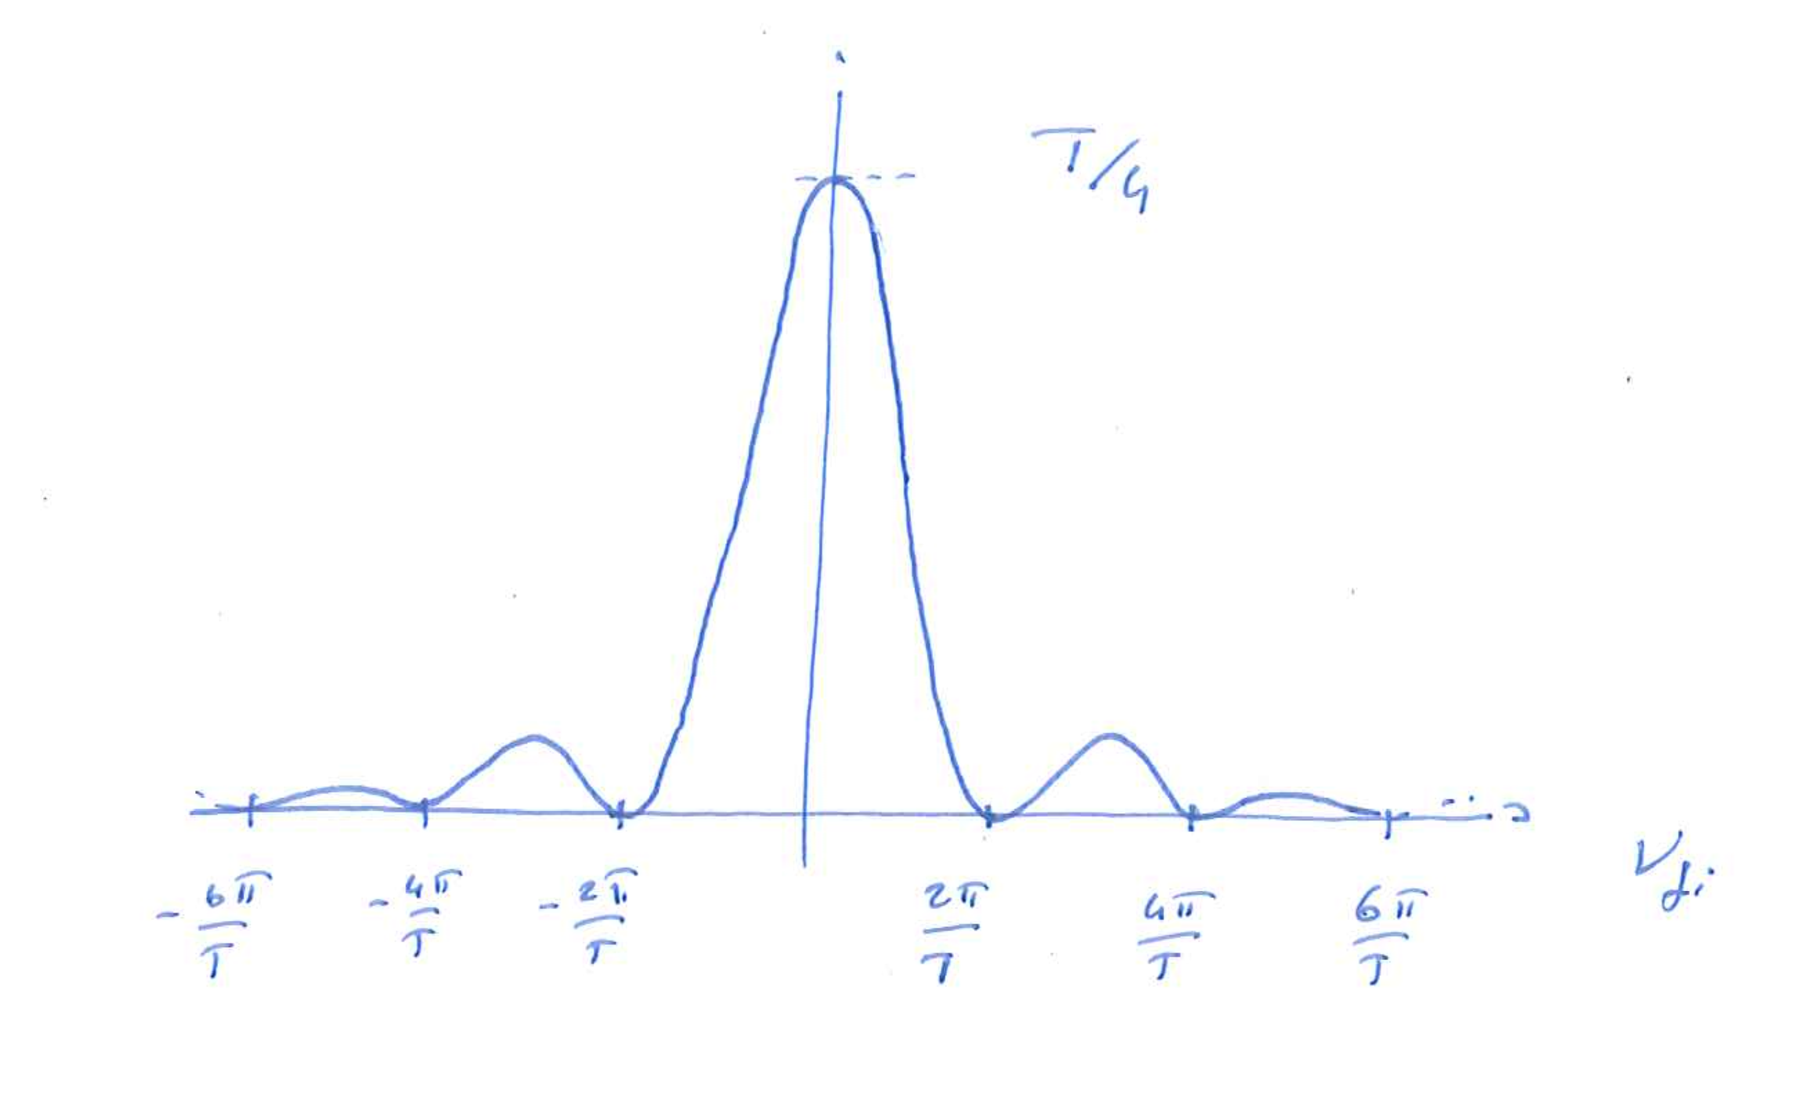
\includegraphics[scale=0.2]{Figures/qscat1.pdf}
    \caption{Evolution of Eq. \eqref{eq:sinusoidalenufi} as a function of the difference between the final and initial state energy $\nu_{fi}$.}
    \label{fig:quantum-scattering:1}
\end{figure}

Let's extend our reasoning to the continuum case, i.e. let's assume that we have a continuum of possible energy states, and that we are interested in the $dn$ accessible states in the range $[E_{f},E_{f}+dE_{f}]$. The total transition rate  can be expressed as a sum of continuous elements $d\Gamma_{fi}$ of transition rates, where
\begin{equation*}
    d\Gamma_{fi} = |T_{fi}|^2\times\frac{1}{T}\int_{-\frac{T}{2}}^{\frac{T}{2}}\int_{-\frac{T}{2}}^{\frac{T}{2}}e^{i(E_{f}-E_{i})t}e^{-i(E_{f}-E_{i})t'}dtdt'dn.
\end{equation*}
Considering long time intervals, $T\rightarrow\infty$, we have
\begin{equation*}
    d\Gamma_{fi} = |T_{fi}|^2\times\lim_{T\rightarrow \infty}\frac{1}{T}\int_{-\frac{T}{2}}^{\frac{T}{2}}\int_{-\frac{T}{2}}^{\frac{T}{2}}e^{i(E_{f}-E_{i})t}e^{-i(E_{f}-E_{i})t'}dtdt'dn.
\end{equation*}
In order to calculate the total rate, we can exploit the fact that the Fourier transform of $1$ is the Dirac delta function, $\delta$,
\begin{equation*}
    \int_{-\infty}^{+\infty}e^{ik(x-x_0)}dk = 2\pi\delta(x-x_0).
\end{equation*}
Therefore we have 
\begin{equation*}
    \int_{-\infty}^{+\infty}e^{i(E_{f}-E_{i})t'}dt' = 2\pi\delta(E_{f}-E_{i}),
\end{equation*}
and we can write the contribution to the total transition rate due to the several accessible states in the $[E_{f},E_{f}+dE_{f}]$ energy range as
\begin{equation*}
    d\Gamma_{fi} = |T_{fi}|^2 dn \lim_{T\rightarrow \infty}\left[\frac{1}{T}\int_{-\frac{T}{2}}^{\frac{T}{2}}e^{i(E_{f}-E_{i})t}dt \right] \times 2\pi\delta(E_{f}-E_{i}),
\end{equation*}
and so the total transition rate can be expressed as
\begin{equation*}
    \Gamma_{fi} = \int d\Gamma_{fi} = \int |T_{fi}|^2 \frac{dn}{dE_{f}}\lim_{T\rightarrow \infty}\left[\frac{1}{T}\int_{-\frac{T}{2}}^{\frac{T}{2}}e^{i(E_{f}-E_{i})t}dt\right]2\pi\delta(E_{f}-E_{i})dE_{f},
\end{equation*}
obtaining, using the delta properties on the integral,
\begin{equation*}
    \Gamma_{fi} = 2\pi\int|T_{fi}|^2 \frac{dn}{dE_{f}}\delta(E_{f}-E_{i})dE_{f}\times \lim_{T\rightarrow \infty} \frac{1}{T}\int_{-\frac{T}{2}}^{\frac{T}{2}}dt.
\end{equation*}

But
\begin{equation*}
    \lim_{T\rightarrow \infty} \frac{1}{T}\int_{-\frac{T}{2}}^{\frac{T}{2}}dt = 1,
\end{equation*}
therefore the total transition rate is written as
\begin{equation*}
    \Gamma_{fi} = 2\pi|T_{fi}|^2\left|\frac{dn}{dE_{f}}\right|_{Ei},
\end{equation*}
where
\begin{equation*}
      \left|\frac{dn}{dE_f} \right|_{E_{i}} = \rho(E_i)
\end{equation*}
is the density of accessible states in the final state, given the initial energy $E_{i}$. We can therefore write the total transition rate as
\begin{equation*}
    \Gamma_{fi} = 2\pi|T_{fi}|^2\rho(E_{i}).
\end{equation*}
For completeness, we report also its expression when $\hslash\neq1$:
\begin{equation*}
    \Gamma_{fi} = \frac{2\pi}{\hslash}|T_{fi}|^2\rho(E_{i}).
\end{equation*}

\section{Fermi's golden rule}
Until now assumed $a_{k\neq i} (t) \sim 0$: what happens if we relax this assumption? Let's take again Eq. \eqref{quantum-scattering:eq2} and keep only the assumption that $a_{i}(t) \sim 1$, and that $V=V(x)$: we have
\begin{equation*}
    i \sum_{k} \frac{\partial a_{k}(t)}{\partial t} \Phi_{k}(\Vec{x})e^{-iE_{k}t} = V(\Vec{x})\Phi_{i}(\Vec{x})e^{-iE_{i}t} + \sum_{k\neq i}  V(\Vec{x})a_{k}(t)\Phi_{k}(\Vec{x})e^{-iE_{k}t}.
\end{equation*}
Multiplying by $\langle f |$ and integrating over the volume $V$, we get
\begin{equation}
\begin{split}
    i\frac{\partial a_{f}(t)}{\partial t} &= \int_{V}d^3x\,\Phi_{f}^*(\Vec{x})V(\Vec{x})\Phi_{i}(\Vec{x})e^{i(E_{f}-E_{i})t} \\&+ \sum_{k\neq i}\int_V d^3x\Phi_f^*(\Vec{x})V(\Vec{x})a_{k}(t)\Phi_{k}(\Vec{x}) e^{i(E_{f}-E_{k})t}.
\end{split}
    \label{quantum-scattering:eq4}
\end{equation}

The strategy to get the solutions to the Schr\"odinger equation in this more general case ($a_{k\neq i} (t) \neq 0$) is to approximate $a_k(t)$ with the solutions from Eq. \eqref{quantum-scattering:eq3} (which were obtained assuming, at the first order, $a_{k\neq i}(t)=0)$: in other words, we write
\begin{equation*}
\begin{split}
    a_{k}(t) &= -i \int_{0}^{T}\left[\int_{V}\Phi_{k}^*(\Vec{x}) V(\Vec{x})\Phi_{i}(\Vec{x})d^3x \right] e^{i(E_{k}-E_{i})t'}dt'\\
    &= -i\frac{e^{i(E_k-E_i)t}}{i(E_k-E_i)}\int_V\Phi_k^*(\Vec{x}) V(\Vec{x})\Phi_i(\vec{x}) d^3x\\
    &= -\frac{e^{i(E_k-E_i)t}}{E_k-E_i} \int_V \Phi_k^*(\Vec{x}) V(\Vec{x})\Phi_i(\vec{x}) d^3x.
\end{split}
\end{equation*}
We then insert this expression in Eq. \eqref{quantum-scattering:eq4}, obtaining 
\begin{equation*}
\begin{split}
    \frac{\partial a_{f}(t)}{\partial t} &= \left[-i\int_{V} d^3x \Phi_{f}^*(\Vec{x}) V(\Vec{x})\Phi_{i}(\Vec{x}) \right] e^{i(E_{f}-E_{i})t} \\
    &+ (-i)(-1) \sum_{k\neq i} \frac{\int_{V}d^3x\Phi_{f}^*(\Vec{x})V(\Vec{x})\Phi_{k}(\Vec{x})\int d^3x\Phi_{k}^*(\Vec{x})V(\Vec{x})\Phi_{i}(\Vec{x})}{(E_{k}-E_{i})} e^{i(E_{k}-E_{i})t} e^{i(E_{f}-E_{k})t}.
\end{split}
\end{equation*}
%since
%\begin{equation*}
 %   a_{k}(t) = -i \int_{V}d^3x \Phi_{k}^*(\Vec{x}) V(\Vec{x}) \Phi_{i}(\Vec{x}) d^3x %\frac{e^{i(E_{k}-E_{i})t}}{i(E_{k}-E_{i})},
%\end{equation*}
%which is, integrating over the time $t'$, the solution at the first order for $a_{k}(t)$.

Using the bra-ket notation,
\begin{equation*}
    \langle f | V | i \rangle = \int_{V}\Phi_{f}^*(\Vec{x})V(\Vec{x})\Phi_{i}(\Vec{x}) d^3x,
\end{equation*}
we can write
\begin{equation*}
    \frac{\partial a_{f}(t)}{\partial t} = -i \left[\langle f | V | i \rangle + \sum_{k\neq i} \frac{\langle f | V | k \rangle\langle k | V | i \rangle}{E_{i}-E_{k}} \right] \times e^{i(E_{f}-E_{i})t}.
\end{equation*}

What we did is effectively to obtain a better approximation of the transition matrix element $T_{fi}$,
\begin{equation*}
    T_{fi} = \langle f|V|i\rangle + \sum_{k\neq i}\frac{\langle f |V|k\rangle\langle k |V|i\rangle}{E_{i}-E_{k}},
\end{equation*}
which is again a time-independent expression. We can insert it in Eq. \eqref{quantum-scattering:eq3}, 
and use this second-order evaluation of $T_{fi}$ in the expression of the Fermi's golden rule. The procedure can be iterated, obtaining more and more precise approximations of the solutions of the Schr\"odinger equation for an arbitrary potential.

\section{Perturbative calculation and particles exchange}\label{sec:perturbativecalc}
This iterative calculation has a fundamental interpretation in particle physics.
We have seen that at second order one has
\begin{equation}\label{eq:reminderTfi}
    T_{fi} = \langle f |V| i\rangle + \sum_{k\neq i}\frac{\langle f|V|k\rangle\langle k |V|i \rangle}{E_{i}-E_{k}}.
\end{equation}
We can see the first-order calculation of a scattering process as a simple scattering within the potential zone, highlighted by a ``bubble'' in Fig. \ref{quantum-scattering:fig2}.
\begin{figure}[h]
    \centering
    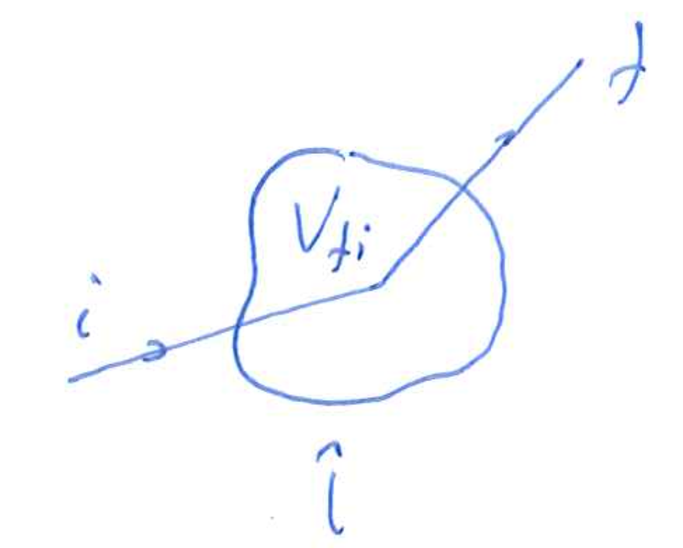
\includegraphics[scale=0.3]{Figures/firstorder.pdf}
    \caption{Picture of a scattering interaction at first order in the perturbative calculation.}
    \label{quantum-scattering:fig2}
\end{figure}
At second order, the interaction happens through an intermediate state $k$, as represented in Fig. \ref{quantum-scattering:fig3}.
\begin{figure}[h]
    \centering
    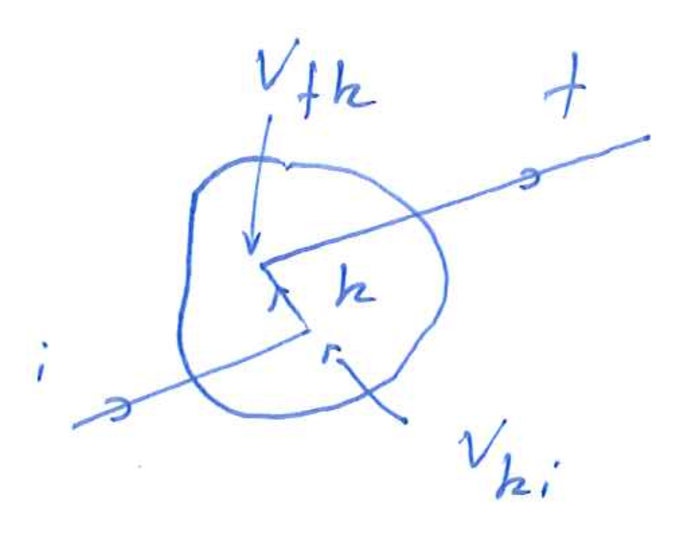
\includegraphics[scale=0.3]{Figures/secondorder.pdf}
    \caption{Picture of a scattering interaction at second order in the perturbative calculation: the scattering happens through an intermediate state $k$.}
    \label{quantum-scattering:fig3}
\end{figure}
The potential describing each interaction is denoted with subscripts, e.g. $V_{fi} = \langle f | V | i \rangle$ for the direct interaction between the initial and final state (same holds for $V_{fk}$ and $V_{ki}$).

In this representation, when a particle is scattered in a potential, there is a  momentum exchange between two particles through the potential, which is called a ``ranged interaction''. If the potential is created by a particle (e.g. a gold nucleus in the Rutherford experiment), during the ranged interaction the potential should  change instantly, but this would not be possible due to special relativity.

A new formulation of the process can be obtained thinking of the interaction as if were mediated by a \emph{mediator particle} $X$, as shown in Fig. \ref{quantum-scattering:fig4}. Let us also include the time in our ``picture'' of an interaction: for example, let's take an interaction $a+b\rightarrow c+d$
\begin{figure}
    \centering
    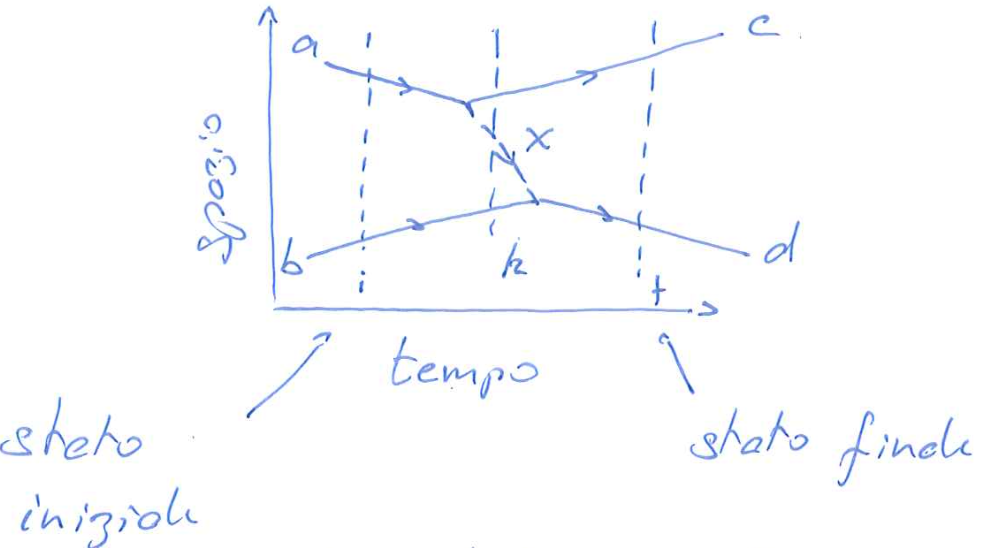
\includegraphics[scale=0.5]{Figures/qscat2.pdf}
    \caption{Picture of a possible, mediated interaction which brings from an initial state of two particles $a+b$ to a final state $c+d$. The horizontal axis represents time, while the vertical axis represents space, and the interaction between particles is mediated by a mediator $X$. In this specific picture, the $a$ particle emits $c$ together with $X$, which is then absorbed by $b$ which emits $d$.}
    \label{quantum-scattering:fig4}
\end{figure}
where the intermediate state is $k$. We will also assume that the interaction is quite simple: the transition matrix between any state is represented by a constant \emph{coupling} $g$, defined as
\[\langle k |V|i\rangle = g=\langle f |V|k\rangle,\]
as shown in Fig. \ref{quantum-scattering:fig5}. In this example, one way in which we can write the initial, intermediate and final states in terms of their particle content is
\begin{equation*}
    i:\,\,a+b,  \,\,\,\,\,\,\,\,\, k:\,\,c+x+b,\,\,\,\,\,\,\,\,\, f:\,\,c+d.
\end{equation*}
We can see this as the following time sequence:
\begin{enumerate}
    \item in the initial state $i$, we have the particles $a$ and $b$;
    \item the intermediate state $k$, where the particle $a$ emits a particle $X$ and a particle $c$, which exist together with $b$;
    \item the final state $f$, where $b$ has absorbed $X$ and emitted $d$, and so we are left only with $c$ and $d$.
\end{enumerate}
    
\begin{figure}[h]
    \centering
    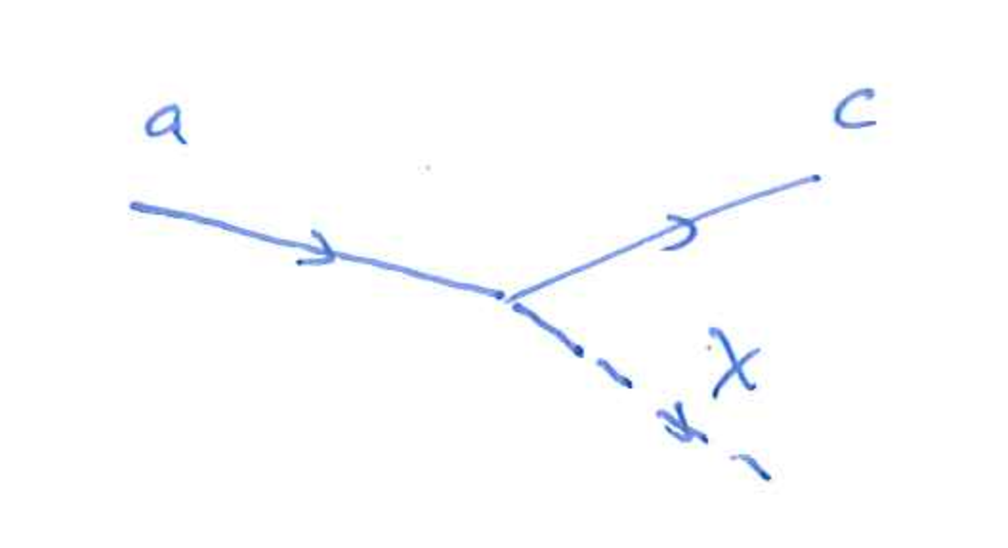
\includegraphics[scale=0.2]{Figures/qscat3.pdf}
    \caption{Simple interaction with a constant coupling $g$ between two quantum states $a$ and $c$; $X$ is the  particle which mediates their interaction (``mediator'').}
    \label{quantum-scattering:fig5}
\end{figure}

In this case, we have the transition matrix element
\begin{equation*}
    T_{fi}^{(i)} = \frac{\langle f | V | k\rangle\langle k | V | i \rangle}{E_{i}-E_{k}},
\end{equation*}
where the superscript $i$ is to remind us that we are considering \emph{one} possible option ($a$ emits $X$ and subsequently $b$ absorbs it).
The energies of the three states, in this specific hypothesis of what's going on in the interaction, are
\begin{align*}
        E_{i} = E_{a}+E_{b},\\
        E_{k} = E_{c}+E_{X}+E_{b},\\
         E_{f} = E_{c}+E_{d}.
\end{align*}
We use the assumption that $V_{lm}=g$ does not depend on the states $l$ and $m$, and write
\begin{equation*}
    T_{fi}^{(i)} = \frac{g^2}{(E_{a}+E_{b}) - (E_{c}+E_{x}+E_{b})} = \frac{g^2}{E_{a}-E_{c}-E_{x}}.
\end{equation*}

But, in the sum of Eq. \eqref{eq:reminderTfi}, we need to consider all possible intermediate states, even the ones in which $b$ emits $X$ and $a$ absorbs it, as it is shown in Figure \ref{quantum-scattering:fig6}. This is a crucial point!
\begin{figure}
    \centering
    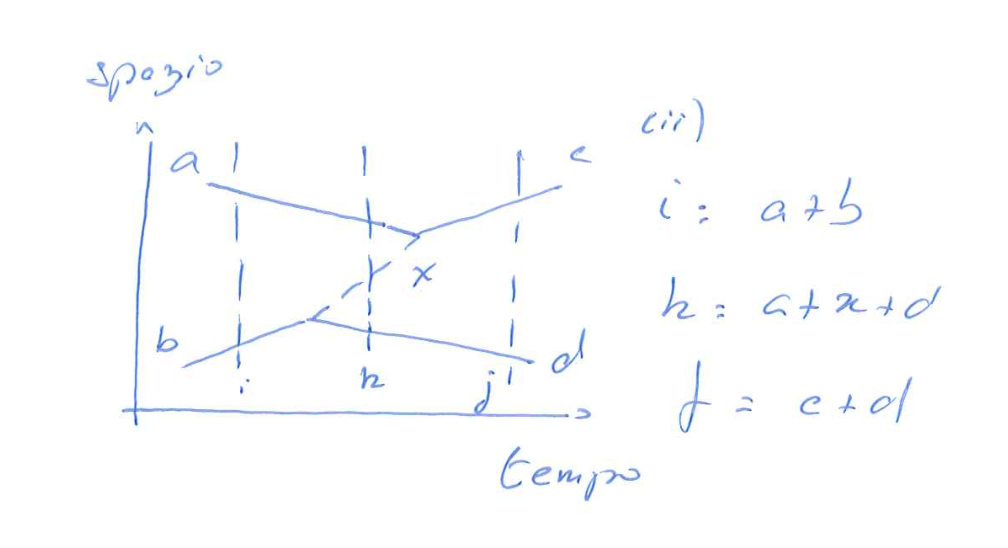
\includegraphics[scale=0.5]{Figures/qscat4.pdf}
    \caption{Picture of an alternative interaction between $a$ and $b$, which leads to a final state $c+d$. In this specific picture, the $b$ particle emits $d$ together with $X$, which is then absorbed by $a$ which emits $c$.}
    \label{quantum-scattering:fig6}
\end{figure}
In this case we have
\begin{align*}
        &E_{i} = E_{a}+E_{b},\\
        &E_{k} = E_{a}+E_{X}+E_{d},\\
         &E_{f} = E_{c}+E_{d},
    \end{align*}
from which one gets
\begin{equation*}
    T_{fi}^{(ii)} = \frac{g^2}{E_b-E_d-E_X},
\end{equation*}
again with a superscript $ii$ which reminds us the fact this is another term in the sum of Eq. \eqref{eq:reminderTfi}.
Since the energy conservation can be written as
\begin{equation*}
    E_a + E_b = E_c + E_d \,\,\,\,\rightarrow\,\,\,\, E_b = E_c + E_d - E_a,
\end{equation*}
we can write
\begin{equation*}
    T_{fi}^{(ii)} = \frac{g^2}{E_c-E_a-E_X}.
\end{equation*}

The sum of these two contributions is
\begin{equation*}
    T_{fi}^{(i)} + T_{fi}^{(ii)} = g^2 \left( \frac{1}{E_a-E_c-E_X} - \frac{1}{E_a-E_c+E_X} \right) = \frac{2g^2E_X}{(E_a-E_c)^2-E_X^2}.
\end{equation*}
From the relativistic energy-momentum-mass relation we can write
\begin{equation*}
    E_X^2 = p_X^2 + M_X^2,
\end{equation*}
where $\Vec{p_X} = \Vec{p_a} - \Vec{p_c}$ (i.e. we assumed the conservation of momentum in the process $a\to X+c$). Therefore,
\begin{equation*}
    E_X^2 = (\Vec{p_a} - \Vec{p_c})^2 + M_X^2.
\end{equation*}

If we define the four-momenta $q$, $p_a$ and $p_c$, we have
\[q = p_a - p_c,\]
from which we can write
\begin{equation*}
    T_{fi} = 2E_X \frac{g^2}{(E_a-E_c)^2 - (\Vec{p_a} - \Vec{p_c})^2 - M_X^2},
\end{equation*}
and since $(E_a-E_c)^2 - (\Vec{p_a} - \Vec{p_c})^2 = q^2$, we have
\begin{equation*}
    T_{fi} = 2E_X \frac{g^2}{q^2-M_X^2}.
\end{equation*}
The term
\begin{equation*}
    \frac{1}{q^2 - M_x^2}
\end{equation*}
is called the \emph{propagator of the interaction}.% (or of the interaction particles).
The term $g$ is called the \emph{coupling} of the interacting particles to the mediator of the interaction itself.

Note that the term $T_{fi}$ is not a Lorentz invariant, due to the presence of the term $2E_X$. The term
\begin{equation*}
    \frac{g^2}{q^2-M^2}
\end{equation*}
is instead a Lorentz invariant. The interaction rate must necessarily not depend on the reference frame we use to describe the interaction, while the term $2E_X$ does depend on the normalisation chosen for the wave functions during the perturbation calculation. In fact, choosing a different normalisation (which in quantum mechanics, we stress it, cannot affect the results of any physical measurements) we can absorb the $2E_X$ term: we can in fact require that the space integral of the free-particle wave functions is
\begin{equation*}
    \int_V \Phi^*\Phi\,d^3x = 2E_X,
\end{equation*}
instead of $1$.

One should also note that it is necessary to maintain the chosen order of perturbation theory for all the considered intermediate configurations of the system.
The higher order of perturbation we apply, the more intermediate configuration are possible; in particular, these two numbers coincide.

\section{Feynman diagrams}
The calculations of cross-sections and decay rates in particle physics is performed using a different formalism in relativistic quantum mechanics and quantum field theory. A representation of the calculations can be given through the use of \emph{Feynman's diagrams}, in which the perturbations which were ordered in time are instead represented by single diagrams, as shown in Fig. \ref{quantum-scattering:fig7}.
\begin{figure}[h]
    \centering
    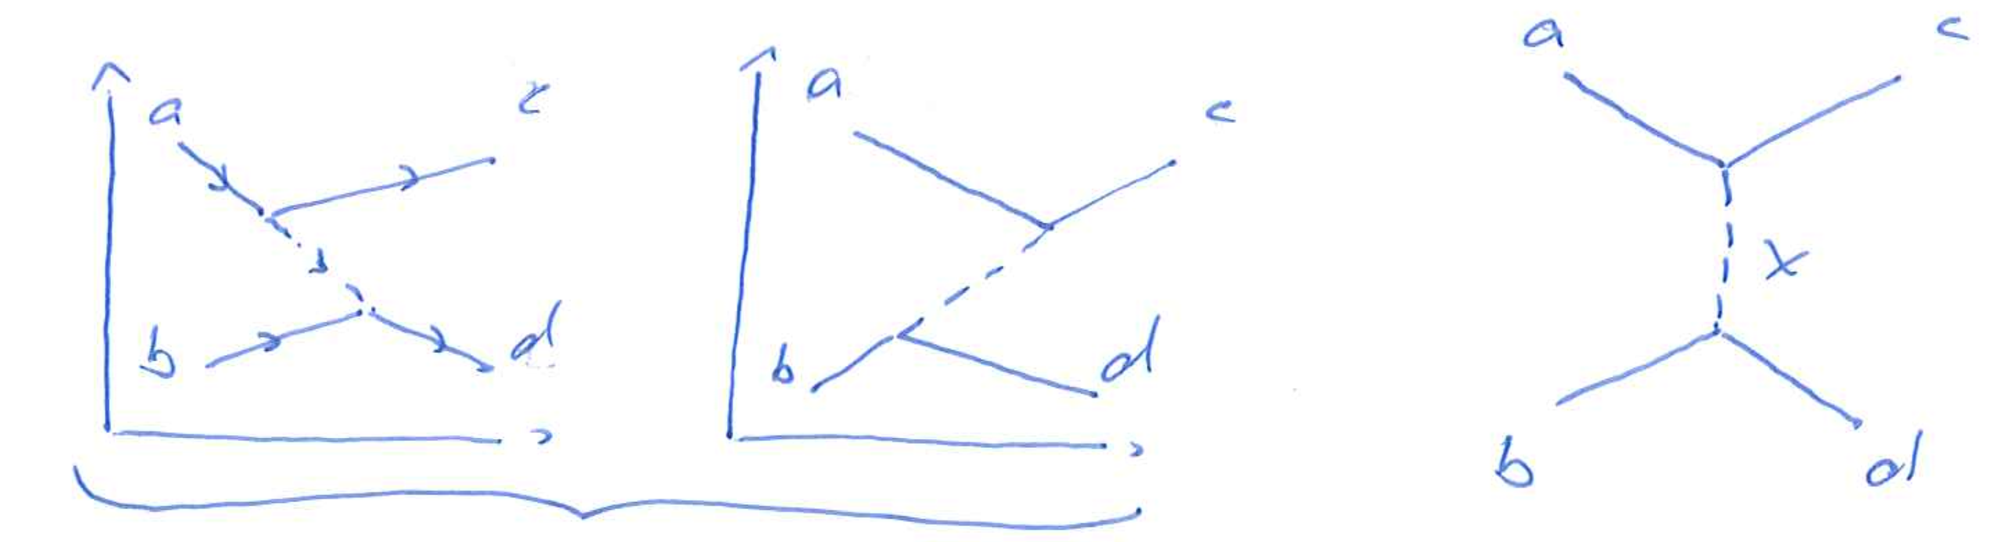
\includegraphics[scale=0.32]{Figures/qscat5}
    \caption{The alternative interactions which were ordered in time in perturbation theory, shown by the left diagrams, are replaced by a single Feynman diagram, shown on the right.}
    \label{quantum-scattering:fig7}
\end{figure}

As shown in the case of perturbation theory, in the interaction ``vertices'' the energy is not conserved and the $X$ particle, the mediator, is considered as a physical particle which may be measured/observed. In the Feynman diagram formalism, instead, the mediator is considered as an ``intermediate'' state with a \emph{virtual mass} $q^2$ which does not correspond to the mass of the free particle, $M_X^2$ ($q^2\neq M_X^2$); but the four-momentum is conserved at the vertices. A virtual particle can be seen as a mathematical construct which represents the sum over all the possible time ordering considered by perturbation theory.

Both representations are equivalent. The ``classical'' interpretation with the exchange of a physical intermediate particle fulfills the interpretation of the momentum transfer.

\section{Density of states, wave function normalisation and phase space}
How can we calculate the density of states, which is needed in order to obtain the transition rate from an initial and a final state according to Fermi's golden rule? We start from the fact that the wave function of a free particle is given by
\begin{equation*}
    \psi(\Vec{x},t) = Ae^{i\Vec{p}\cdot\Vec{x}-iEt},
\end{equation*}
and its normalisation is usually obtained requiring
\begin{equation*}
    \int_{V}d^3x \psi^*\psi = 1,
\end{equation*}
which corresponds to one particle in the volume $V$. This is an important element to consider. In the case of a free particle (plane wave), in a cubic volume $V$ with side $a$ (i.e. a box) we therefore have
\begin{equation*}
    \int_0^a\int_0^a\int_0^a\psi^*\psi\,dx\;dy\;dz\, = 1.
\end{equation*}
The normalisation of the wave function $A$ is therefore
\begin{equation*}
    A^2 = \frac{1}{a^3} = \frac{1}{V}.
\end{equation*}
This normalisation implies that the wave function satisfies the boundary conditions 
\begin{equation*}
    \psi(x+a,y,z) = \psi(x,y,z) = \psi(x,y+a,z) = \psi(x,y,z+a).
\end{equation*}
Taking a volume $V$ with periodic boundary conditions is equivalent to the case of  wave functions which vanish at the borders of a box, but allows easier calculations with momenta.

We want to count the number of possible states for given energy or momentum. Let's start with momentum: the periodic boundary conditions applied to the $x$ direction imply that
\begin{equation*}
    e^{ip_xx} = e^{ip_x(x+a)},
\end{equation*}
and similarly for the $y$ and $z$ directions. Therefore, from the requirement $e^{ip_xa} = 1$ we have that $p_xa$ must be a multiple of $2\pi$; this implies
\begin{equation*}
    (p_x,p_y,p_z) = \frac{2\pi}{a}(n_x,n_y,n_z),
\end{equation*}
where $n_x, n_y, n_z$ are integers.
In other words, not all momentum values are allowed, and the momentum space is quantized, as shown in Fig. \ref{quantum-scattering:fig8}.
\begin{figure}[h]
%    \centering
    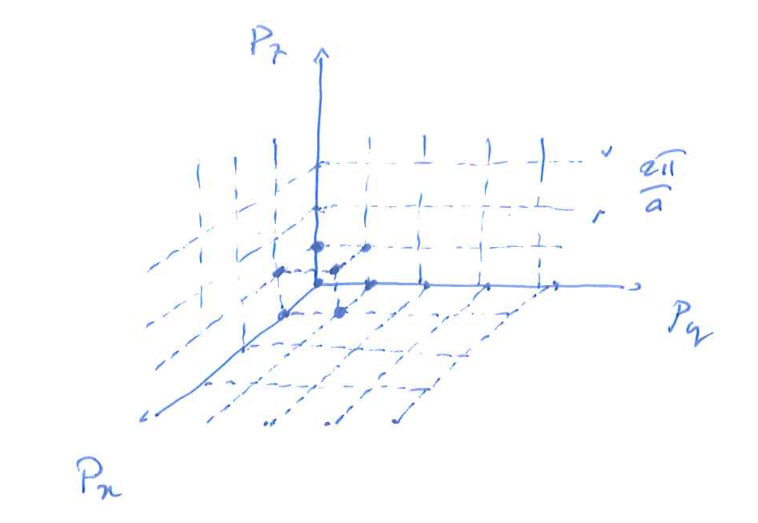
\includegraphics[scale=0.36]{Figures/qscat6}
    \caption{Quantization of the momentum space. Any particle lives in a point of this three-dimensional grid.}
    \label{quantum-scattering:fig8}
\end{figure}

In order to count the number of states with momentum in the range $[p,p+dp]$, we have to perform a calculation over a 3D sphere in the $(p_x,p_y,p_z)$ space;  Fig. \ref{quantum-scattering:fig9}  shows a projection of this sphere on the $(p_x,p_y)$ plane.
\begin{figure}[h]
    \centering
    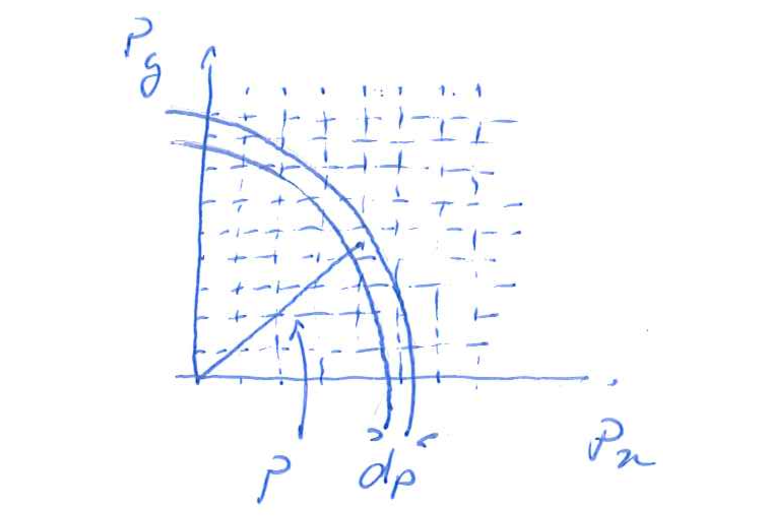
\includegraphics[scale=0.4]{Figures/qscat7}
    \caption{Projection over the $(p_x,p_y)$ plane of the quantisation of the space of the momenta.}
    \label{quantum-scattering:fig9}
\end{figure}
Every single state occupies a cubic volume
\begin{equation*}
    d^3p = dp_x\,dp_y\,dp_z\, = \left(\frac{2\pi}{a}\right)^3 = \frac{(2\pi)^3}{V},
\end{equation*}
therefore the number of states with momentum $p \in [p,p+dp]$ will be equal to the ratio between the volume between two spheres with a radius differing by $dp$, $4\pi p^2dp$, divided by the volume occupied by a single state:
\begin{equation*}
    dn = 4\pi p^2 dp\left(\frac{V}{(2\pi)^3}\right).
\end{equation*}
This leads to
\begin{equation*}
    \frac{dn}{dp} = \frac{4\pi p^2}{(2\pi)^3}V.
\end{equation*}
We can in turn write the density of states as
\begin{equation}\label{eq:dennedp}
    \rho(E) = \frac{dn}{dE} = \frac{dn}{dp}\left|\frac{dp}{dE}\right|.
\end{equation}
From the last term of the right-hand side of this equation, one can see that decays to lighter particles are more probable (have higher density of states) than decays to heavier particles.

Again, the interaction rate will not depend on the overall normalisation, which cancels out with the other terms from Fermi's golden rule: the normalisation of the waveform is $1/\sqrt{V}$, and its square appears in the transition matrix element squared, which cancels out with the factor $V$ in Eq. \eqref{eq:dennedp}.
To simplify the calculations we can take therefore an unitary volume, $V=1$, choosing a normalisation which corresponds to one particle per volume unit.

For a solid angle element $d\Omega$, the density of the states can be expressed using spherical coordinates as\footnote{We simply used the fact that the volume element in spherical coordinates is $r^2drd\Omega=r^2dr\sin\theta d\theta d\phi$.}
\begin{equation*}
    dn = p^2\sin{\theta}\,dpd\theta d\phi \frac{V}{(2\pi)^3},
\end{equation*}
therefore
\begin{equation*}
    \frac{dn}{dp} = \frac{p^2\sin{\theta}dpd\theta d\phi}{(2\pi)^3}V.
\end{equation*}
For a final state with $N$ particles, there will be $N-1$ independent momenta (due to momentum conservation), therefore we need to count $N-1$ final states:
\begin{equation*}
    dn = \prod_{i=1}^{N-1}dn_i = \prod_{i=1}^{N-1}\frac{d^3p_i}{(2\pi)^3}V.
\end{equation*}

In the case of a decay of a particle into $N$ particles, $a\to b_1+b_2+\dots + b_n$, the number of independent states can be expressed in terms of all $N$ particles in the final state, by using a Dirac delta to impose the conservation of momentum:
\begin{equation*}
    dn = (2\pi)^3\prod_{i=1}^{N}\frac{d^3p_i}{(2\pi)^3}\delta^3\left(\vec{p}_a-\sum_{i=1}^N \vec{p}_i\right) V.
\end{equation*}

\section{Cross-section and decay rate}
The concept of cross section is related to the transition rate (or interaction rate) in the case of a beam of particles $A$ which interact with a target of particles $B$, through the relation
\begin{equation*}
    \frac{dN_i}{dt} = \sigma\Phi_A N_B,
\end{equation*}
where $\Phi_A$ is the flux of $A$ particles, and $N_B$ is the number of targets accessible to the beam. Considering a particle density $n_A$ and a velocity of the beam $v_A$, we have seen that one can write
\begin{equation*}
    \Phi_A = n_A v_A.
\end{equation*}
The cross-section is the equivalent surface for a single particle target of the interaction
\begin{equation*}
    \sigma = \frac{1}{\Phi_A N_B}\times \frac{dN_I}{dt}.
\end{equation*}

The rate $\Gamma_{fi}$ is defined by the Fermi's golden rule: for a specific scattering corresponds to
\begin{equation*}
    %\frac{d\sigma}{d\Omega}
    \sigma= \frac{\Gamma_{fi}}{\Phi_A} = \frac{2\pi}{\hslash}\frac{|T_{fi}|^2\rho(E_{i})}{\Phi_A},
\end{equation*}
and depends on $\rho(E_i)$ (the density of states, a function of the initial state energy $E_i$) and $\Phi_A$, which must be evaluated correctly.

In the case of particle decays, instead, the decay rate $\Gamma_{fi}$ is directly given by Fermi's golden rule.

\section{Electromagnetic interaction - the Rutherford scattering}
Let's consider a simple case for which we know the classical cross-section, the Rutherford scattering, which is the scattering of a charged particle by an electrostatic potential
\begin{equation*}
    V_{C}(r) = \frac{Ze}{4\pi\epsilon_0r}.
\end{equation*}
Our goal is to compute the cross-section in quantum mechanics, using the time-dependent perturbation theory we developed in the last sections.

Let us consider again a beam of  $\alpha$ particles, with a charge $Ze$, mass $m$ and momentum $\Vec{p_i}$. Given the typical energy of $\alpha$ particles, the problem -- as we have seen -- is non-relativistic.
 We will choose a normalisation of the wave function corresponding to $1$ particle per unit volume, so that we will have $n_A = 1$, and $\Phi_{A} = v_{A} = \frac{p_i}{m}$. We will call $\Vec{p}_f$ the final state momentum and $\theta$ the angle between the initial and final directions of the momentum (the ``scattering angle'').
\begin{figure}[h]
    \centering
    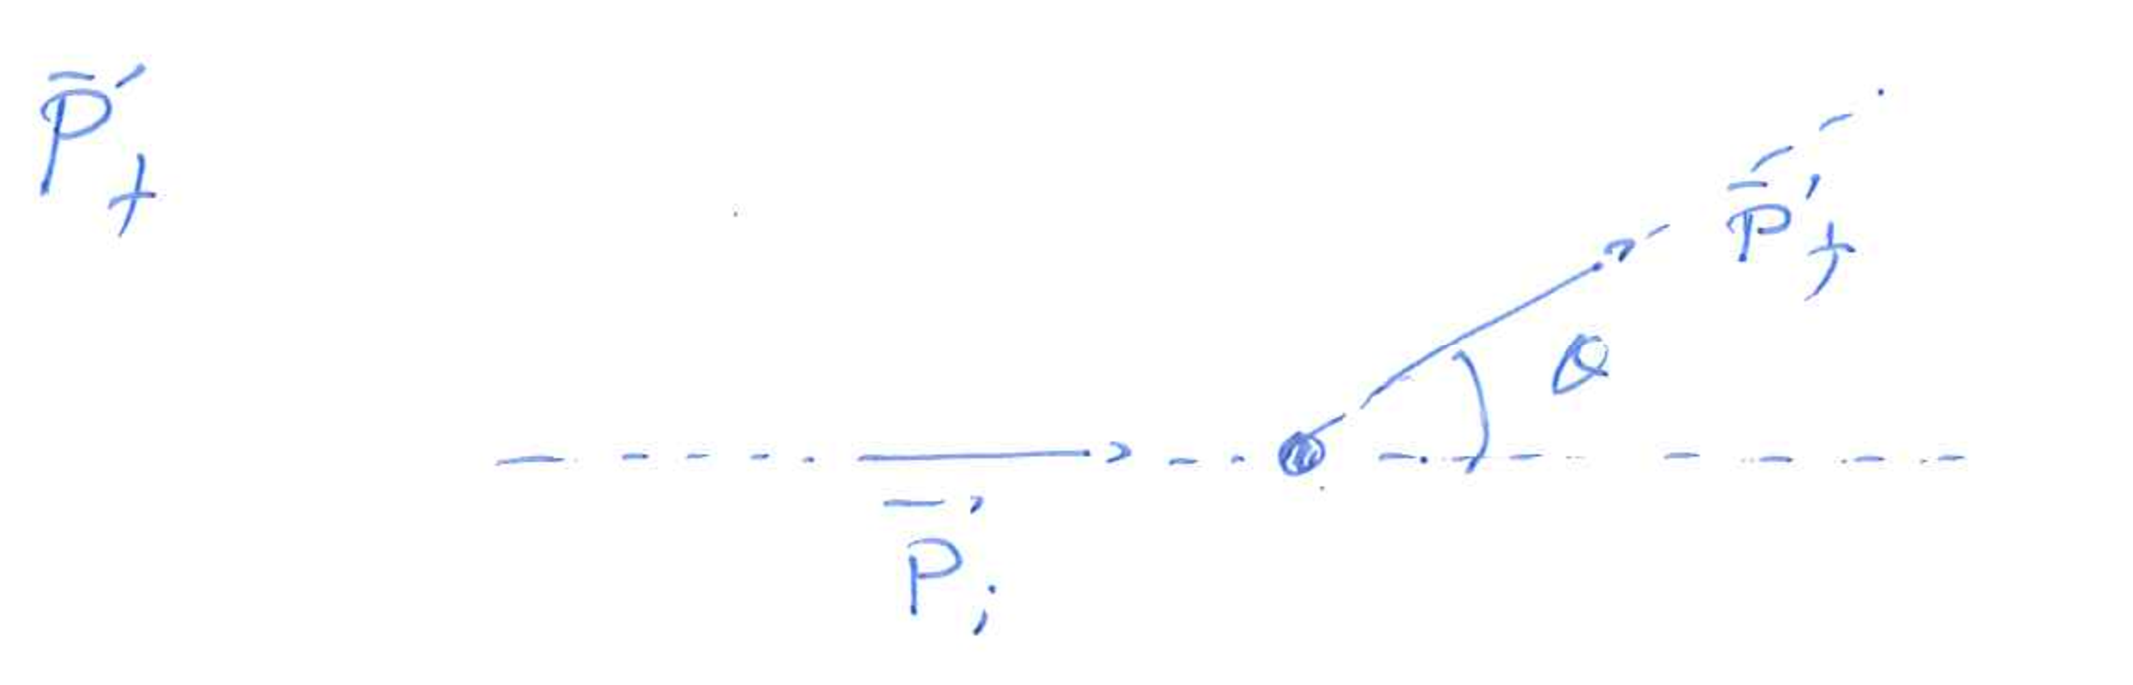
\includegraphics[scale=0.25]{Figures/qscat8}
    \caption{Relation between initial and final state momenta and scattering angle of an $\alpha$ particle in the Rutherford scattering experiment.}
    \label{fig:qscat-fig8}
\end{figure}

Fermi's golden rule is
\begin{equation*}
\Gamma_{fi} = \frac{2\pi}{\hslash} |T_{fi}|^2 \rho(E_i),
\end{equation*}
where $\rho(E_{i})$ is the density of the final states (given the initial state energy) included in the solid angle $d\Omega_f$. We have
\begin{equation*}
    \frac{dn}{dp} = \frac{p^2\sin{\theta}d\theta d\phi}{(2\pi)^3},
\end{equation*}
and since in the initial and final state the $\alpha$ particle is free, we have
\begin{equation*}
    E_{f} = \frac{p_f^2}{2m},
\end{equation*}
so that we can write
\begin{equation*}
    \frac{dE_f}{dp_f} = \frac{p}{m}.
\end{equation*}

The wave functions of the initial and final states, normalised to $1$, are
\begin{equation*}
    \psi_i = e^{i(\Vec{p_i}\cdot\Vec{r} - Et)}\;\;\;\;\;\;\;\psi_f = e^{i(\Vec{p_f}\cdot\Vec{r}-Et)},
\end{equation*}
therefore
\begin{equation*}
    T_{fi} = \int_{V}d\Vec{x} \psi_{f} V(r)\psi_i.
\end{equation*}
Note that in this case $V(r)$ is the \emph{potential energy}, not the Coulomb potential:
\begin{equation*}
    V(r) = -ze\frac{Ze}{4\pi\varepsilon_0 r}.
\end{equation*}
Using the conservation of energy ($E_f=E_i$), we obtain
\begin{equation*}
    T_{fi} = -\frac{zZe^2}{4\pi\varepsilon_0}\int_{0}^{\infty}\int_{0}^{\pi}\int_{0}^{2\pi}r^2\sin{\tilde{\theta}}e^{i\Vec{q}\cdot\Vec{r}}\frac{1}{r}drd\tilde{\theta}d\phi,
\end{equation*}
where $\Vec{q} = \Vec{p_i} - \Vec{p_f}$, and $\tilde{\theta}$ is the polar angle in the direction $\Vec{q}$ (not to be confused with the polar scattering angle $\theta$).

Therefore, we can write
\begin{equation*}
    \frac{-zZe^2}{4\pi\varepsilon_0}\int_{0}^{\infty}\int_{0}^{\pi}\int_{0}^{2\pi}r^2\sin{\tilde{\theta}}e^{iqr\cos\tilde{\theta}}\frac{1}{r}drd\tilde{\theta}d\phi.
\end{equation*}
We define $y = \cos{\tilde{\theta}}$, so that we have
\begin{equation*}
    dy = -\sin{\tilde{\theta}}d\tilde{\theta},
\end{equation*}
and then performing the integral over $\phi$, obtaining
\begin{equation*}
    T_{fi} = \frac{zZe^2}{4\pi\varepsilon_0}2\pi\int_{0}^{\infty}\int_{-1}^{-1}r^2e^{iqry}\frac{1}{r}drdy = \frac{zZe^2}{4\pi\varepsilon_0}2\pi\int_{0}^{\infty}r\left[\int_{-1}^{1}e^{iqry}dy\right]dr.
\end{equation*}

Since
\begin{equation*}
    \int_{-1}^{1}e^{iqry}dy = \frac{e^{iqr}-e^{-iqr}}{iqr} = 2\frac{\sin{(qr)}}{qr},
\end{equation*}
we have (assuming $\hslash=c=1$)
\begin{equation*}
    \begin{split}
        T_{fi} & = \frac{zZe^2}{4\pi\varepsilon_0}2\pi\int_{0}^{\infty}\frac{2i}{qi}\sin{(qr)}dr = 4\pi zZ\alpha\frac{1}{q}\int_{0}^{\infty}\sin(qr)dr = \\
        & = 4\pi zZ\alpha \frac{1}{q}\left[\frac{e^{iqr}+e^{-iqr}}{iq\cdot2i}\right]_{0}^{\infty}.
    \end{split}
\end{equation*}

We can consider that the potential is shielded for large enough distances, and therefore introduce a term $e^{-\varepsilon r}$ for which we take
\begin{equation*}
    \frac{1}{r}\rightarrow \lim_{\varepsilon\rightarrow0}\frac{e^{-\varepsilon r}}{r}.
\end{equation*}
The oscillating term in the integral we need to solve to calculate $T_{fi}$ becomes
\begin{equation*}
    \lim_{\varepsilon\rightarrow 0}\int_{0}^{\infty}e^{-\varepsilon r}\sin{(qr)}dr = \lim_{\varepsilon\rightarrow 0}\left[\frac{e^{iqr-\varepsilon r}}{(iq-\varepsilon )2i}-\frac{e^{-iqr-\varepsilon r}}{(-iq-\varepsilon)2i}\right]_{0}^{\infty},
\end{equation*}
so
\begin{equation*}
    \lim_{\varepsilon\rightarrow 0}\int e^{-\varepsilon r}\sin{qr} dr = \lim_{\varepsilon \rightarrow 0}\frac{q}{q^2+\varepsilon^2} = \frac{1}{q},
\end{equation*}
and in the end we get
\begin{equation*}
    T_{fi} = 4\pi\alpha z Z \frac{1}{q^2}.
\end{equation*}
We get the given form of the matrix element which includes the product of two numbers, $ze$ and $Ze$ (``couplings''), and a ``\emph{propagator}" of the form $\frac{1}{q^2-M_X^2}$, where $M_X = 0$ (the massless photon).
The transferred momentum can be expressed as
\begin{equation*}
    q^2 = |\Vec{p_i} - \Vec{p_f}|^2 = 2p_i^2(1-\cos{\theta}),
\end{equation*}
where $p_i = p_f$ (in general the scattering is elastic and the nucleus does not move), and $p_i^2 = p_f^2 = 2mE$ ($E$ is the kinetic energy of the $\alpha$ particle), therefore
\begin{equation*}
    q^2 = 8mE\sin^2\left(\frac{\theta}{2}\right),
\end{equation*}
where we used
\begin{equation*}
    1-\cos{\theta} = 2\sin^2\left(\frac{\theta}{2}\right).
\end{equation*}

For the cross section we have
\begin{equation*}
    d\sigma = \frac{\Gamma_{fi}}{\Phi_A} = \frac{2\pi|T_{fi}|^2\rho(E_i)}{p_i/m},
\end{equation*}
where 
\begin{equation*}
    \rho(E_i) = \frac{p_i^2\sin{\theta}d\theta d\phi}{(2\pi)^3}\times\left(\frac{dp}{dE}\right) = \frac{p_i^2d\Omega}{(2\pi)^3}\frac{m}{p_i}.
\end{equation*}
The differential cross-section can then be written as
\begin{equation*}
    \frac{d\sigma}{d\Omega} = \frac{1}{(2\pi)^2}T_{fi}^2m^2 = \frac{1}{(2\pi)^2}(4\pi)^2\times(\alpha zZ)^2\times\frac{1}{64E^2\sin^4\frac{\theta}{2}},
\end{equation*}
and in the end
\begin{equation*}
    \frac{d\sigma}{d\Omega} = \frac{(\alpha zZ)^2}{16}\frac{1}{E^2\sin^4\frac{\theta}{2}},
\end{equation*}
which is the Rutherford cross section, the same of the classical calculation!

\section*{Take-home lessons}
\begin{itemize}
    \item One of the keys of scattering theory is that we consider particles at infinite distance from the region where a potential acts as \emph{free particles}, which can then be described with plane waves, i.e. positive-energy solutions of the free-particle Schr\"oedinger equation. Negative-energy solutions instead represent (in non-relativistic quantum mechanics) bound states.
    \item In quantum mechanics, a different choice on the normalisation of a wave function must have no effect on calculated physical quantities (like cross-sections). Probability current can then be interpreted in terms of the flux of particles of a beam.
    \item In time-independent perturbation theory (i.e. if the Hamiltonian of a system does not depend on time), and in the presence of a central potential in a three-dimensional space, it is convenient to express the Schr\"oedinger equation in terms of the sperical expression of the Laplacian operator $\nabla^2$. In this way, its solutions can be separated into a radial and an angular part. The wave function can then be expanded in partial waves, i.e. projected onto the basis formed by the Legendre polynomials: one finds that a plane wave can ve decomposed into two spherical waves, one propagating outwards and one inwards. 
    \item In general, the Hamiltonian of a system may depend on time, and one would have to use the time-dependent perturbation theory to get an approximated solution of the Schr\"oedinger equation. The solution to this equation can be expressed in the basis of the solutions of the free-particle Hamiltonian, in terms of coefficients which are time-dependent. If the perturbative potential is weak, one can find an expression of the transition probability between two states of the system (which in the end is a concept related to the scattering cross-section!), and use this to calculate the total transition probability. This latter quantity in turn depends on the density of accessible states.
    \item If one brings time perturbation theory to second order, one can see (Fermi's Golden Rule) that the transition matrix between the initial and final state depends on a sum over possible intermediate states $k$, so that the transition $i\to f$ is actually $i\to k \to f$. This sum should run over \emph{all} possible intermediate states: an interaction $a+b\to c+d$ can then be seen as mediated by the exchange of another particle $x$, which implies a contribution to the transition matrix which depends on its mass $M_x$ and on a coupling strength factor $g$ which "weighs" the interaction with $x$.
    \item Feynman diagrams represent a convenient way to visualize this summation over possible intermediate states. They prove essential to compute cross-sections in Relativistic Quantum Mechanics and Quantum Field Theory.
    \item The density of states represents the volume density of accessible states in the momentum space. It is a quantity which depends on energy-momentum conservation -- a final state with $N$ particles will have only $N-1$ independent momenta, as the total momentum is constrained to be equal to the initial state value.
    \item The Golden Rule allows to express the interaction rate in terms of the square of the transition matrix between initial and final state, and of the density of states.
    \item The quantum-mechanical calculation of the differential cross-section of Rutherford scattering yields the same results as the classical calculation.
\end{itemize}
\section*{Questions}
\begin{itemize}
    \item In quantum mechanics, are energy eigenvalues always quantised?
\end{itemize}
